\documentclass[12pt,a4paper]{scrartcl}
\usepackage[ngerman]{babel}
\usepackage[T1]{fontenc}
\usepackage[utf8]{inputenc}
\usepackage[paper=a4paper,left=25mm,right=25mm,top=25mm,bottom=15mm]{geometry}
\usepackage{graphicx}
\usepackage[automark]{scrlayer-scrpage}
\usepackage[german=guillemets]{csquotes}
\usepackage{minitoc}
\usepackage{mwe}
\usepackage{tocloft}
\usepackage{lipsum}
\usepackage{longtable}
\usepackage{setspace}
\usepackage{moreenum}
\usepackage{caption}
\captionsetup{labelformat=empty}
\usepackage{wrapfig}
\usepackage{amsmath}
\usepackage{multicol}
\usepackage{floatrow}
\usepackage{marvosym,xcolor}
\definecolor{dorgreen}{HTML}{33B200}
\definecolor{mygreen}{rgb}{0,0.6,0}
\definecolor{mygray}{rgb}{0.5,0.5,0.5}
\definecolor{mymauve}{rgb}{0.58,0,0.82}
\usepackage{verse}
\usepackage[version=4]{mhchem}

\usepackage{listings}
\renewcommand\lstlistingname{Code-Auszug}
\lstset{
  backgroundcolor=\color{white},   % choose the background color; you must add \usepackage{color} or \usepackage{xcolor}
  basicstyle=\fontsize{9}{11}\selectfont,        % the size of the fonts that are used for the code
  breakatwhitespace=false,         % sets if automatic breaks should only happen at whitespace
  breaklines=true,                 % sets automatic line breaking
  captionpos=t,                    % sets the caption-position to bottom
  commentstyle=\color{mygreen},    % comment style
  deletekeywords={...},            % if you want to delete keywords from the given language
  escapeinside={\%*}{*)},          % if you want to add LaTeX within your code
  extendedchars=true,              % lets you use non-ASCII characters; for 8-bits encodings only, does not work with UTF-8
  frame=single,	                   % adds a frame around the code
  keepspaces=true,                 % keeps spaces in text, useful for keeping indentation of code (possibly needs columns=flexible)
  keywordstyle=\color{blue},       % keyword style
  otherkeywords={*,...},            % if you want to add more keywords to the set
  numbers=left,                    % where to put the line-numbers; possible values are (none, left, right)
  numbersep=5pt,                   % how far the line-numbers are from the code
  numberstyle=\tiny\color{mygray}, % the style that is used for the line-numbers
  rulecolor=\color{black},         % if not set, the frame-color may be changed on line-breaks within not-black text (e.g. comments (green here))
  showspaces=false,                % show spaces everywhere adding particular underscores; it overrides 'showstringspaces'
  showstringspaces=false,          % underline spaces within strings only
  showtabs=false,                  % show tabs within strings adding particular underscores
  stepnumber=2,                    % the step between two line-numbers. If it's 1, each line will be numbered
  stringstyle=\color{mymauve},     % string literal style
  tabsize=2,	                   % sets default tabsize to 2 spaces
  title=\lstname                   % show the filename of files included with \lstinputlisting; also try caption instead of title
}

\lstset{literate=
  {á}{{\'a}}1 {é}{{\'e}}1 {í}{{\'i}}1 {ó}{{\'o}}1 {ú}{{\'u}}1
  {Á}{{\'A}}1 {É}{{\'E}}1 {Í}{{\'I}}1 {Ó}{{\'O}}1 {Ú}{{\'U}}1
  {à}{{\`a}}1 {è}{{\`e}}1 {ì}{{\`i}}1 {ò}{{\`o}}1 {ù}{{\`u}}1
  {À}{{\`A}}1 {È}{{\'E}}1 {Ì}{{\`I}}1 {Ò}{{\`O}}1 {Ù}{{\`U}}1
  {ä}{{\"a}}1 {ë}{{\"e}}1 {ï}{{\"i}}1 {ö}{{\"o}}1 {ü}{{\"u}}1
  {Ä}{{\"A}}1 {Ë}{{\"E}}1 {Ï}{{\"I}}1 {Ö}{{\"O}}1 {Ü}{{\"U}}1
  {â}{{\^a}}1 {ê}{{\^e}}1 {î}{{\^i}}1 {ô}{{\^o}}1 {û}{{\^u}}1
  {Â}{{\^A}}1 {Ê}{{\^E}}1 {Î}{{\^I}}1 {Ô}{{\^O}}1 {Û}{{\^U}}1
  {œ}{{\oe}}1 {Œ}{{\OE}}1 {æ}{{\ae}}1 {Æ}{{\AE}}1 {ß}{{\ss}}1
  {ű}{{\H{u}}}1 {Ű}{{\H{U}}}1 {ő}{{\H{o}}}1 {Ő}{{\H{O}}}1
  {ç}{{\c c}}1 {Ç}{{\c C}}1 {ø}{{\o}}1 {å}{{\r a}}1 {Å}{{\r A}}1
  {€}{{\EUR}}1 {£}{{\pounds}}1
}

\renewcommand{\cftpartleader}{\cftdotfill{\cftdotsep}}
%\renewcommand{\cftchapleader}{\cftdotfill{\cftdotsep}}
\renewcommand{\cftsecleader}{\cftdotfill{\cftdotsep}}

\chead{- \thepage \hspace{1pt} - }
\cfoot{}

 \makeatletter
 \def\xdotfill{\@ifnextchar[{\@xdotfilli}{\@xdotfilli[0.5ex]}}
 \def\@xdotfilli[#1]#2{%
 \@ifnextchar[{\@xdotfillii[#1]{#2}}{\@xdotfillii[#1]{#2}[black]}}
 \def\@xdotfillii[#1]#2[#3]{%
 \leaders
 \hbox{\raisebox{#1}{\color{#3}\rule{1.2pt}{#2}\kern 1.5pt}}\hfill%
 \color{black}}
 \makeatother

\let\raggedpart\centering
\makeatletter
\@addtoreset{section}{part}
\makeatother

%\renewcommand*{\partheadmidvskip}{\nobreakspace}
\renewcommand*{\partformat}{\thepart}

\newcommand*{\extendedpart}[5]{
% 1: Betreff; 2: Titel; 3: Zusammenfassung; 4: Bild; 5: Autor
\begin{titlepage}
\begin{large}
    \centering
    #1\par
    % Entweder:
    \addpart{#2}\refstepcounter{part}
    % Oder 
     %\part{#2}
    \vfill
    #3\par
    \vfill
    #4\par
    \vfill
    \textbf{Autor:} #5\par
  \end{large}
  \end{titlepage}
  %\parttoc
}

\usepackage{hyperref}

\hypersetup{pdfinfo={
  Title=Pibel,
  Author=Der allmächtige Schöpfer N,
  Subject=Dabendorf Glaubensbuch,
  Keywords={Dabendorfismus, Dabendorf, Pibel, Glaubensbuch, Maltismus-Dabendorfismus, Papst, Konsul, Prinzessin, Einhorn}}
}
%\makeindex
%\usepackage[numberedsection,toc]{glossaries}\makeglossaries

%\newglossaryentry{n}{name=N,description={Unser großer Freund und Helfer N}}
%\newglossaryentry{mephisto}{name=Mephistopheles,description={Der schreckliche Antagonist des N: Mephistopheles, kurz Mephisto}}
%\gls{n} im Dokument verbreiten

\begin{document}
\extendedpart{Nationalbibliothek der Dabendorf Orthodoxen Kirche}{Pibel}{Der große Glaubensalmanach der Dabendorf Orthodoxen Religion}{
\includegraphics[width=.7\textwidth]{bilder/doreinhornTitle.jpg}}{Der allmächtige Schöpfer \textit{N}}

\setcounter{tocdepth}{3}
\tocloftpagestyle{empty}
%\doparttoc
\tableofcontents

%Einleitende Worte, Begriffe, Dabendorf, Franzakenreich, DORgötter
\clearpage
\section{{Einleitende Worte des N}}
Wenige Jahre nach dem Untergang des repressiven Kapitalistenregimes vor einigen Milliarden Sekunden ist dieses Buch durch unseren allmächtigen Schöpfer \textit{N} publiziert worden, um der Bevölkerung Halt und neuen Glauben in der Umsetzung des großen Plans eines geeinten und glücklichen Dabendorfs zu geben. Es dient als großer Glaubensalmanach für all diejenigen, die sich dem großen Dabendorftum, der \textit{Dabendorf Orthodoxen Religion} angeschlossen haben, um die Idee des \textit{Maltismus-Dabendorfismus} und die Lehren des \textit{N} neu aufleben zu lassen. Die Grundlagen dieses Schriftstücks werden auf ewig die Macht der Dabendorfer Bevölkerung über ihr eigenes Leben sichern und große Unterdrückungsmuster in der Gesellschaft besiegen können. In all diesen Wünschen und Träumen unterstützt uns \textit{N}, der große Initiator unseres neuen Weltbilds, der über uns schwebt und uns stets mit hilfreichen Denkanstößen zur Seite steht. \textit{N} ist Ideengeber einer großartigen Religion, die sich durch ihren friedvollen, prokrastinativen und gedankenreichen Ansatz von allen Vorgängerreligionen im Grundsatz unterscheidet. Das Glaubenswerk des \textit{N} löst in unwissenden oder gar christlichen Menschen jedoch einen sehr denkintensiven und Gehirnschmalz kostenden Prozess aus, der zu schweren Nebenwirkungen führen und die Leser geistig vernichten kann. Der Schmöker ist auf eigene Gefahr zu lesen. Dies ist die magische Funktion des Buches, welche Ungläubige genau identifizieren und nachhaltig prägen kann.

\section{{Begriffserläuterung}}
Die Dabendorf Orthodoxe Religion wird mit der in Kapitälchen stehenden Dreibuchstabenkombination \textit{DOR} abgekürzt. Sie wird in der allgemein-gültigen Grammatik in allen Fällen nach normalen Regeln abgekürzt. Die Einwohner Dabendorfs nennen sich \textit{Dabendorfer}, die Menschen, die den Glauben der Dabendorf Orthodoxen Religion vertreten sind allesamt \textit{DORs}. Allen Substantiven, die eine Verbindung zur DOR herstellen, wird selbige Abkürzung vorangestellt, wie beispielsweise der \textit{DORpapst} oder die \textit{DORzeit}. Die Einwohner der Hauptstadt Dabendorf Citys nennen sich \textit{Erzdabendorfer}. Einwohner des \textit{Franzakenreich} genannten Nachbarstaats Dabendorfs nennen sich \textit{Franzaken}.

\section{{Topographie des Sonnentrabanten Erde}}
Die Dabendorf Orthodoxe Bevölkerung lebt auf einem Trabanten des Sterns Sonne, als dessen Bezeichnung sich die Wortschöpfung \textit{Erde} eingebürgert hat. Die Erdmassen des gesamten Planeten sind zum Großteil frei von unnötigen politischen Grenzziehungen, sodass nahezu einhundert Prozent der Bevölkerung der Erde im \textit{Weltstaat Dabendorf} lebt. Lediglich im Westen einer geographischen Bezeichnung namens \textit{Europa} hat sich ein Staat mit gegensätzlicher Ideologie entwickelt - das \textit{Franzakenreich}. Die beiden Staaten leben in vollständigem Frieden und unterhalten freundschaftliche Beziehungen zueinander.

\subsection{{Dabendorf}}
Der Weltstaat Dabendorf umfasst neunundneunzig Prozent der Erdmasse und ist neben dem Franzakenreich die einzige geopolitische Gliederung der Erde. Die Einwohner dieses Staats werden als Dabendorfer bezeichnet. Sie alle sind frei und gleich und unterliegen keiner repressiven Macht, wie es in Systemen wie dem Kapitalismus üblich ist. Der große Staat Dabendorf wird von der Hauptstadt Dabendorf City aus durch das Konklave der drei DORpäpste regiert, welche sich in zwei Konsule und eine Prinzessin unterteilen.

\subsection{{Dabendorf City}}
Die Hauptstadt Dabendorfs, die in vorherigen Herrschaften nur als Dabendorf bekannt war, trägt den Namen \textit{Dabendorf City}. Sie beherbergt den Dabendorfer Herrschaftspalast mit der großen \textit{Prinzessin HaNNa} und die meisten großen Pilgerstätten der Dabendorf Orthodoxen Religion, in welchen selbige ihren großen Ursprung fasste und \textit{N} seine erste \textit{Banane mit Salz} aß. In ihr leben die \textit{Erzdabendorfer}, welche eine besondere Bindung zur Religion aufweisen können.

\subsection{{Das Franzakenreich}}
Das \textit{Franzakenreich} ist ein junger Staat, der sich nach dem Untergang des Kapitalistenregimes der alten Welt auf dem Gebiet des damaligen Frankreichs bildete und weiterhin die Ideologie des Kapitalismus vertritt. Er ist die einzige Landmasse, die nicht zum \textit{Weltstaat Dabendorf} gehört und mit selbigem im Gegensatz steht. Die Völker Dabendorfs und des Franzakenreichs unterhalten jedoch freundschaftliche Beziehungen zueinander und sind dem Gedanken sich gegenseitig zu bekriegen vollkommen abgeneigt. Der weitgehende Pazifismus auf beiden Seiten ist der Grund für den andauernden Frieden auf der \textit{Erde}. Autoritärer Herrscher des Franzakenreichs ist der mit ebenfalls allmächtigen Kräften bestückte \textit{Napoléon Bonaparte}, welcher durch ein \textit{Baguetteduell} auf den Herrschaftsthron des Landes gelingen konnte. Das Franzakenreich lebt vollkommen andere Bräuche und kulturelle Inhalte als Dabendorf, hat sich jedoch als gleichberechtigter Verhandlungspartner in allen weltrelevanten Fragen entwickelt. Es unterhält innerhalb Dabendorfs eine kleine Exklave in der Stadt \textit{Kleinfrankreich}, in welcher sich die \textit{Franzakische Botschaft} befindet. Gegensätzlich dazu befindet sich ein kleines burgundisches Dorf namens \textit{Taizé} im Dabendorfer Staatsbesitz, welches sich seit Jahrhunderten für die Völkerverständigung zwischen den Einwohnern Dabendorfs und des Franzakenreichs einsetzt.

\section{{Die drei DORgötter}}
Der Dabendorf Orthodoxe Glaube basiert auf einem System der Götter, welches sich aus drei essentiellen Hauptgöttern und zahlreichen Nebengöttern zusammensetzt. Selbige Götter haben das Dabendorfer Leben seit ewigen Zeiteinheiten entscheidend geprägt und werden dies bis zum Untergang des Universums durch das Szenario \textit{Big Jane} auch weiterhin entschlossen tätigen. Das politische, wirtschaftliche und gesellschaftliche Gleichgewicht der Dabendorf Orthodoxen Welt und ihrer Satellitenwelten ist einzig und allein abhängig von den Launen des \textit{Triumphats der großen drei DOR-Götter}. Die Unmengen an Dabendorf Orthodoxen Nebengöttern fungieren als Chaosschaffende auf unzähligen Nebenkriegsschauplätzen, welche nur in einer Symbiose untereinander einen etwaigen Einfluss auf die großen DOR-Mächte verüben können. Innerhalb der folgenden Kapitel dieser Pibel, dem offiziellen Glaubensbuch der Dabendorf Orthodoxen Religion, werden die Eigenschaften dieser Götter umfangreich dokumentiert und festgehalten. Teile ihrer Eigenschaften sind aufgrund ihrer Mächtigkeit noch nicht hinreichend erforscht worden.
\clearpage
\subsection{{N - Schöpfer unseres Dabendorfs}}
Unser großer Imperator \textit{N} ist der Dabendorf Orthodoxe Hauptgott, welcher die \textit{Dabendorf Orthodoxe Religion}, das Universum, \textit{Dabendorf} als solches, den \textit{Dabendorfer Staat} und all seine Gegebenheiten und Einwohner erschaffen hat. Alle seitdem in diesen Geltungsbereichen stattgefunden habenden Änderungen sind zu einhundert Prozent auf selbigen, seine Anhänger oder andere Hauptgötter zurückzuführen. Eine \textit{Evolution} als solche hat zu keinem Zeitpunkt der Dabendorfer Geschichte stattgefunden, da alle \textit{Commits} auf das menschliche Erbgut stets von \textit{N} ausgeführt wurden. Seine Bezeichnung beruht auf der eigenen \textit{Faulheit}, seinen Namen aufschreiben zu müssen, sowie der Tatsache, dass Statistiken zufolge sein Name bereits vorher in einhundert Prozent der Schriftstücke auftauchte. \textit{N} ist die Antwort auf all unsere Fragen und der mächtige Gegenbuchstabe des \textit{P}. Er ist der wirtschaftspolitische und ideologische Gegner des Mephistopheles der Dabendorfer Unterwelt. \textit{N} ist jedoch nicht wie der Gott anderer sogenannter Religionen vollkommen allmächtig und jederzeit überall. Sein großer Hang zur \textit{Prokrastination} und seine Leidenschaft zum \textit{Schachspiel} sind es, die ihn hindern, sich mit relevanten Beschäftigungen zu befassen. Er ist jedoch immer antreffbar, wenn man in Not gerät.

\subsection{{Mephistopheles - Regent der Sporthallen}}
\textit{Mephistopheles} ist der große Herrscher der Sporthallen, in einer seiner Erscheinungen von Beruf \textit{Sportlehrer} und der große Antagonist des \textit{N}. Er lebt in der Unterwelt, noch weit tiefer als die Tunnel des Vietcong. Alles obskur seltsame, welches augenscheinlich nicht aus dem Franzakenreich stammt, geht von seiner skandalösen Persönlichkeit aus und wird durch die Mächte des \textit{N} wieder ausgeglichen. Die Eindämmung der Kämpfe zwischen \textit{N} und ihm ist die Hauptaufgabe des mächtigen Napoléons des Franzakenreichs. Ferner ist er ebenfalls der Charakter der \textit{Schlange aus dem n-ten Buch des Schöpfers}, welche den Dabendorfer zur \textit{Verführung} an der \textit{Hallorenkugel} brachte. Sein Stimmorgan ist mächtiger und lauter, als alle je in Dabendorf gemessenen Schallwellen.

\subsection{{Napoléon - Herrscher des Franzakenreichs}}
\textit{Napoléon Bonaparte} ist der äußerst relevante dritte Part des dreigliedrigen Dabendorfer Göttersystems. Er ist die anpassungsfähigste Persönlichkeit aller \textit{DOR-Götter} und taucht in allen Geschlechtsformen, Erscheinungsbildern, Aggregatzuständen und teilweise auch an mehreren Orten gleichzeitig auf. Er verkörperte in seinen weit mehr als 42.000 Lebenszyklen bereits Menschen wie \textit{Napoléon Bonaparte}, \textit{Robespierre}, \textit{Ludwig XIV.}, \textit{Ludwig XVI.}, \textit{Bismarck} oder \textit{Charles de Gaulle} und lieh ihnen seinen Charakter. Er ist Regent des Dabendorfer Gegenreichs, dem \textit{Franzakenreich} sowie seiner Exklave \textit{Kleinfrankreich}. Er ist ultimativer Verfechter des sogenannten \textit{Franzakentums} und im Machtgefüge dieser Welt der wahrscheinlich essentiellste Bestandteil. Bedingt durch den Kampf des \textit{Mephistopheles} gegen \textit{N} dient er als Sicherheitsgarantie für die gesamte Welt, indem er als ständiger Vermittler tätig ist und seine Macht gegen größere Konflikte der beiden richtet. Gemäß der sogenannten \textit{Götterungleichung} ist jedoch kein Gott mächtiger als die Summe der Macht der beiden anderen Götter, sodass er mit dem Franzakenreich selbst nicht fähig ist, Dabendorf zu übernehmen und derartige Versuche bereits eingestellt hat. Napoléon leidet jedoch an \textit{chronischen Stimmungsschwankungen}, welche er regelmäßig auf dem Rücken von Schülern der Franzakischen Sprache, die er höchstpersönlich unterrichtet, austrägt. Der Palast des Napoléons wird durch mächtige, nach Hunden aussehende Geschöpfe bewacht, die er mit \textit{Augenbrauen} versucht zu ernähren. Das Palastinnere ist um \textit{int.max} größer von innen, als es von außen an Erscheinung trägt.

%\section{Grüßkultur}

%Politische Gliederung, DORrepräsentanten, Maltismus-Dabendorfismus, Kapitalkritik
\clearpage
\section{{Politische Gliederung Dabendorfs}}
\begin{figure}[!h]
\centering
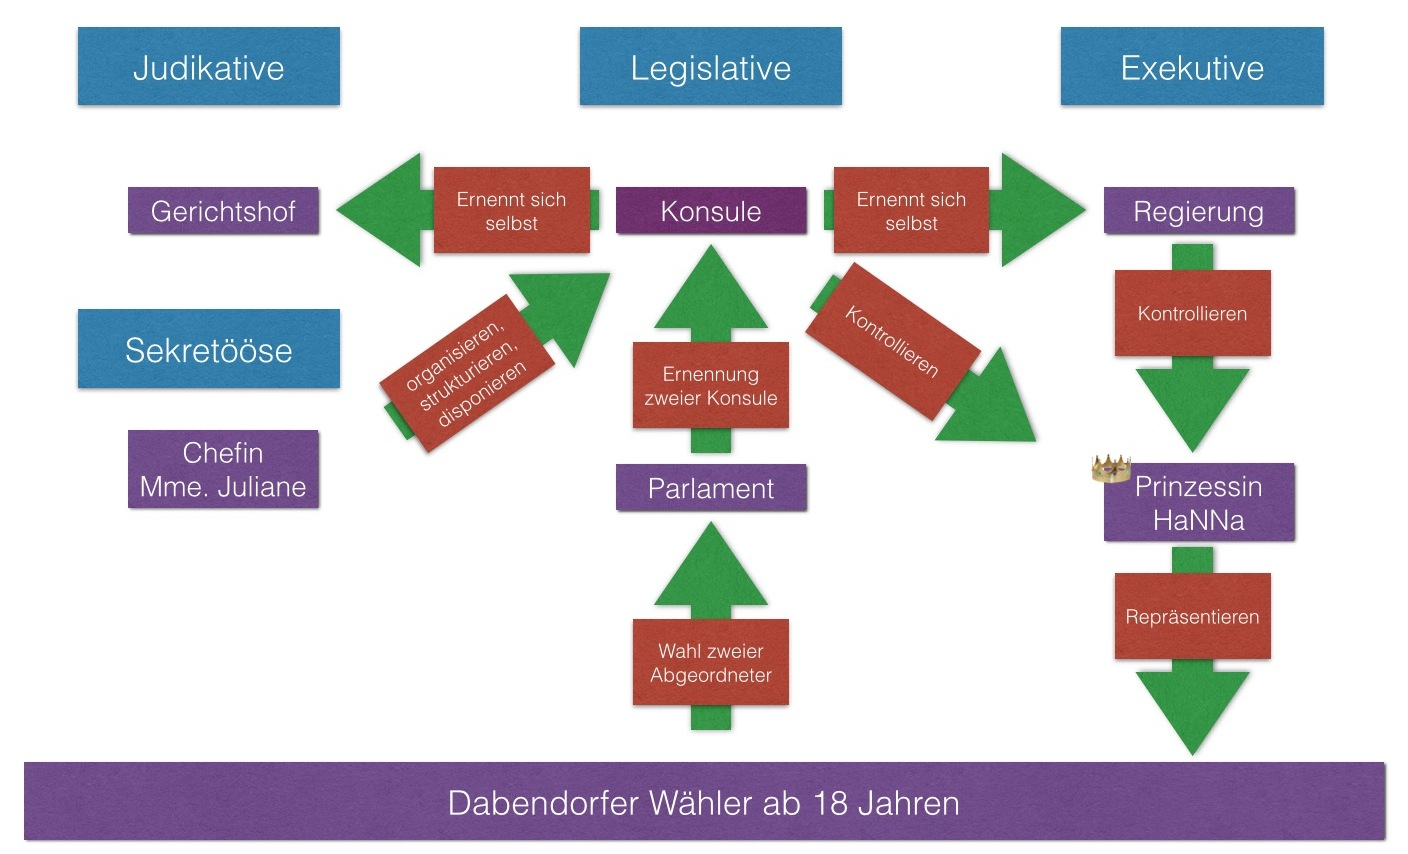
\includegraphics[width=0.95\textwidth]{bilder/gewaltenteilung.jpg}
\caption{Staatsaufbau Dabendorfs nach Gewalten}
\end{figure}
\noindent Der \textit{Dabendorfer Staat} besitzt einen hochkomplexen und in vielen Millionen Zeiteinheiten durch \textit{N} entwickelten Staatsaufbau, der durch seinen \textit{bürokratiearmen}, aber zugleich \textit{höchst effektiven Stil} im Gegensatz zu früheren Systemen und dem System im \textit{Franzakenreich} heraussticht. Eine \textit{Gewaltenteilung} nach den Theorien von Baron de Montesquieu wurde in seriöserer Art und Weise \textit{modifiziert} und umfasst nun neben der \textit{Legislative, einer Exekutive und der Judikative auch die Dabendorfer Sekretööse}, welche alle relevanten \textit{Aufgaben in Dabendorf verwaltet und ausführt}. Das System und seine Mitglieder werden alle \textit{42 Trillionen Jahre durch Wahlen bestätigt}, bei denen alle \textit{Dabendorfer Wähler ab 18 Jahren wahlberechtigt} sind. Wähler Dabendorfs sind alle \textit{mehrzelligen Lebensformen des Planeten Erde}, die \textit{keine Franzakische Staatsbürgerschaft} besitzen. Die Begrenzung des Wahlalters auf 18 Jahre ist ein Relikt früherer Zeiten, als es noch Kinder in Dabendorf gegeben hat. Das Wahlintervall von 42 Trillionen Jahren hat sich aus der Tatsache heraus ergeben, dass \textit{Dabendorfer unsterblich} sind (siehe \textit{\nameref{todsterben}}) und sich kleinere Intervalle als verwaltungstechnisch ineffektiv gezeigt haben. Die \textit{Wähler Dabendorfs wählen} zu den stattfindenden Wahlen insgesamt \textit{zwei Abgeordnete für das Parlament Dabendorfs}. Selbiges \textit{Parlament wählt aus den zwei Abgeordneten insgesamt zwei Abgeordnete} nach einer Kampfabstimmung aus ($\binom{2}{2}$), welche fortan die \textit{Konsule Dabendorfs} darstellen. Die \textit{Konsule Dabendorfs besitzen alle Gewalt der Gesetzgebung in Dabendorf}. Da sie jedoch per definitionem \textit{prokrastinativ arbeitsfern} sind, geben sie ihre Kompetenzen an andere Gewalten ab. Sie bilden die \textit{Dabendorfer Regierung} und kontrollieren die \textit{Prinzessin von Dabendorf}\footnote{Prinzessin von Dabendorf ist ein Eigenname und stammt aus der Zeit vor der Regelung der weiblichen Sprachformen des Dabendorferischen. Der korrekte Term würde in Neudabendorfer Sprache daher \enquote{Prinzööse von Dabendorf} heißen.}. Selbige ist durch \textit{N} höchstpersönlich ernannt worden und \textit{repräsentiert das Dabendorfer Volk}. Die \textit{Prinzessin von Dabendorf} bildet mit den \textit{beiden Konsulen} zusammen die \textit{Päpstliche Dabendorfer Kammer}. Die Konsule sitzen ferner auch im \textit{Dabendorfer Gerichtshof}, treffen alle ihre Entscheidungen jedoch im \textit{Konsensprinzip mit N}. Die eigentlichen \textit{Amtsgeschäfte Dabendorfs} führt jedoch die \textit{Sekretööse} aus, welche im Auftrag der Konsule \textit{organisiert, strukturiert und disponiert}. Sie wird durch die Dabendorfer Konsule nach einem \textit{Dabendorfweiten Casting} im Anschluss an die aktuellen Wahlen ernannt. Es wird jedoch hervorgehoben, dass die Mitglieder des Dabendorfer Verwaltungsapparates \textit{keinerlei Privilegien} zum restlichen Volk besitzen, keine obskuren Extragehälter beziehen und für die \textit{Umsetzung des Volkes Willen} verantwortlich sind.

\subsection{{Die drei Päpste}}
Die \textit{beiden Konsule und die Prinzessin von Dabendorf} bilden zusammen im Namen des \textit{N} die \textit{drei Dabendorfer Päpste}. Sie sind für die \textit{direkte Kommunikation des Volkes}, deren Vertreter sie sind, \textit{mit den großen Dabendorfer Göttern} verantwortlich. Sie besitzen einen direkten Draht zum großen \textit{N}, sind jedoch auch im Stande, innerhalb kürzester Zeit \textit{Kontakt zu Napoléon Bonaparte des Franzakenreichs} aufzunehmen. Sie fungieren als Vertreter des \textit{N} auf Erden, besitzen jedoch \textit{keinerlei außerordentlichen Fähigkeiten}, die \textit{N} besitzt. Ferner sind sie \textit{Verwalter des nationalen Süßkramvorrats} und dafür verantwortlich, dass jeder Bürger Zugriff darauf erhält, ohne dass feindliche Mächte selbigem Schaden zufügen können. Ihr Hauptsitz ist in der \textit{Dabendorf Orthodoxen Kathedrale in Dabendorf City}, in welche sie sich oft einige Zeitintervalle zur individuellen \textit{Prokrastination} zurückziehen.

\subsection{{Die zwei Konsule}}
Die \textit{Dabendorfer Konsule} sind direkt durch das vom Volk gewählte Parlament legitimiert und bilden die \textit{Regierung Dabendorfs}, deren Aufgaben sie an Handlanger und ihre große \textit{Sekretööse von Dabendorf} weitergeben. Sie sind dem \textit{Maltismus-Dabendorfismus} verschrieben und beauftragt, den \textit{Willen des Volkes} umzusetzen. Sie sind die \textit{Gesichter einer antikapitalistischen Regierung}, frei vom Einfluss anderer obskurer Religionen. Nach ihrem \textit{Sieg bei den Wahlen Dabendorfs} sind sie per Gesetz verpflichtet, dem gesamten Wahlvolk einen \textit{Vorrat von Kaffee, Hallorenkugeln und anderem Süßkram} zu verschaffen, der bis zur nächsten Wahl ausreichend vorliegt. Additional dazu ist es ihre \textit{Verantwortung, an jedem Dabendorfer Feiertag} durch den \textit{offiziellen Dabendorf Orthodoxen Gottesdienst} zu führen und den \textit{Segen des N} auf alle Individuen zu verteilen. Eine ihrer wichtigsten Aufgaben ist es auch, \textit{diplomatische Beziehungen zum Franzakenreich} aufzubauen und zu pflegen, sowie den \textit{Staatshaushalt Dabendorfs im Sinne des Maltismus-Dabendorfismus zu verwalten} und \textit{von Kapitalismus und Korruption fernzuhalten}.\\
Amtierende \textit{Konsule von Dabendorf} sind \textit{Malte und Lukas von und zu Dabendorf City}, unterstützt durch ihre \textit{zauberhaften Gattöösen Franzi und Nathi}.

\subsubsection{{Gattööse Nathi}}
Die \textit{ultimativ süß-knuffige Nathi} ist die \textit{liebevoll putzige Gattööse des Papstes Lukas von Dabendorf City}, die seit mehreren Millionen Dabendorfer Zeiteinheiten liebevoll an seiner Seite agiert. Ihr \textit{Verhältnis zu Einhörern ist positiv bis knorke} und ihre \textit{Knuffigkeit grenzenlos}. Sie besitzt das \textit{Dabendorfer Diplom der Meisterstochastikerin} und ist die erste Person der DOR, bei welcher eine \textit{Redegeschwindigkeit} mit reichhaltigem Inhalt gemessen wurde, die \textit{schneller als ein durchschnittlicher Wasserfall} bei $9,81 \frac{m}{s^2}$ Fallbeschleunigung ist. Ferner ist sie \textit{Halterin zahlreicher Dabendorfer Sportrekorde} und konträr zu ihrem Gatten und der Dabendorfer Allgemeinheit durch spezifisch obskure Gene zu \textit{athletischen Höchstleistungen fähig}. Die Limes der \textit{ehelichen Liebe tendiert gegen unendlich} und ermöglicht die einmalige Produktion einer gigantischen Menge an \textit{Bussys}, mit denen das Dabendorfer Volk versorgt und \textit{grenzenlos glücklich} gehalten wird. Ihr spezifisch skandalöser \textit{Hang zum Konsum obskurer Serieninhalte} des \textit{bösen Unkle Sams} sind es jedoch, die ihren Gatten in große Angst versetzen und bestürzend \textit{gruselige Essenz in die Ehe fusionieren}.

\subsubsection{{Gemahlin Franzi}}
\textit{Genossin Franzi} ist die fabulöse \textit{Angetraute des Papsts und Konsuls Malte}, welche in einer streng geheimen Nacht-und-Nebel-Aktion in den \textit{abtrünnigen Gebieten Schottlands} unter mysteriösen Umständen in eine \textit{Ehe} mit selbigem integriert wurde. Sie vertritt \textit{antagonistische Eigenschaften zum Dabendorfer Papst Malte} und ist daher stets für Momente zuständig, die die Dabendorfer Konsule in ihren Grundfesten erschüttern. So vertritt sie \textit{Kreativität, Pünktlichkeit und Opportunismus} in gleich schockierendem Maße und ist auf ähnlich \textit{antiprokrastinativen Wegen} wie die Sekretööse Jane unterwegs. Ferner ist sie \textit{kaffeeabhängig} und vertritt die \textit{künstlerisch-kreativ-musikalische Ebene Dabendorfs}, zumindest diejenige, die nicht schon durch die \textit{phänomenale Raffinesse von Malte und Lukas} abgedeckt ist. Überdies ist additional zu erwähnen, dass sie die magische Gabe besitzt, über einen längeren Zeitraum neben \textit{Dabendorfer Geistlichen} zu sitzen und \textit{Integrale sowie Binomialverteilungen} zu knacken, ohne skandalös zu scheitern.

\subsection{{Prinzessin HaNNa}}
Die \textit{Dabendorfer Prinzessin besitzt repräsentative Zwecke} im Staate und erscheint auf allen relevanten \textit{staatlichen Feiertagen} zur \textit{Zelebration mit dem Dabendorfer Volk}. Sie ist durch \textit{N} höchstpersönlich ernannt und bewegt sich \textit{reitend auf dem Dabendorfer Einhorn Kathi} fort, um ihren zerstörten Rücken instand zu halten. In ihren \textit{Haaren} bewahrt sie allerlei relevanten Krimskrams auf, da sie ein Verfassungsvermögen von über \textit{42 Kubikeiffelturmhöhen} haben. Sie besitzt als einzige Person das \textit{staatlich anerkannte Apfelkuchendiplom} und vertreibt ihre \textit{Apfelkuchen zum Nulltarif} in der großen Kantine des \textit{Dabendorfer Schlosses}, in welchem sie auch residiert. Zu jedem essentiellen Ereignis tritt sie morgens auf dessen Balkon und \textit{wirft Süßkram in die jubelnde Menge}. Sämtliche ihrer \textit{Klamotten} werden durch den \textit{Dabendorfer Stardesigner Malte höchstpersönlich aus roter und DORgrüner Wolle handgehäkelt} und spezialangefertigt. Sie ist die \textit{meist gegooglete Person des Dabendorfer Staates und besitzt Kultstatus in Dabendorfer Souvenirläden}. Amtierende Prinzessin von Dabendorf ist \textit{Ihre Königliche Majestät Prinzessin Mademoiselle HaNNa Elfriede CoriNNa Tebartz von und zu Dabendorf City}. Die Tatsache, dass sie bisher über \textit{keinen Prinzen} verfügt ist der Grund, warum landesweit nach dem bestpassenden männlichen Pendant gesucht wird. Qualifiziert auf selbiges Amt sind nach Definition des \textit{N} jedoch nur diejenigen, die neben den \textit{Konsulen Malte und Lukas} nach dem \textit{Dabendorfer Beziehungsalgorithmus} zu mindestens 99\% der \textit{Prinzessin} zugehörig sind. Ferner muss er im Stande sein, die \textit{Dabendorfer Konsule} und \textit{N} in \textit{mindestens zwei der drei Disziplinen Schach, Bankbowling und Bridge zu besiegen}. Die \textit{Legende} besagt, dass dieser Mensch nur \textit{einmal auf der Erde existiert}, von seinem Glück aber selbst noch nichts weiß. Die Suche des \textit{Prinzen von Dabendorf} beschäftigt mehrere \textit{hundert Wissenschaftler in ganz Dabendorf}.

\clearpage

\subsection{{Einhorn Kathi}}
Das \textit{Dabendorfer Einhorn Kathi} ist das \textit{zauberhafteste Wesen Dabendorfs}, neben den \textit{großen drei Göttern der DOR}. Es ist \textit{persönlicher Begleiter der Prinzessin HaNNa} und für ihre \textit{Sicherheit und den Transport ihrer Person} zuständig. Das Einhorn trägt \textit{pinkes, gut gepflegtes Fell, einen langen DORgrünen Schweif und das große Horn auf dem Kopfe}. Außerdem besitzt es im \textit{Bauch} einen großartigen, \textit{magischen Ofen}, welcher im Stande ist, auf Knopfdruck in kürzester Zeit \textit{Unmengen an Apfelkuchen und Pizza zu produzieren}. Über selbigen Kreislauf ist das Einhorn auch fähig, sich selbst \textit{ohne Energieaufnahme mit Nahrung zu versorgen}. Es ist daher das einzige Wesen auf der Welt, welches dem \textit{Energieerhaltungssatz vehement widerspricht}. Die \textit{Herkunft der Kathi} ist durch eine \textit{geheimnisvolle Legende der Dabendorfer Mythologie überliefert}, welche eines der größten \textit{Rätsel des Dabendorfismus} darstellt. Auf einem großen \textit{DORgrünen Feld hinter der Hauptstadt Dabendorf City} befindet sich ein \textit{großer Kreis mit 42 versteinerten Einhörnern} und einer \textit{kleinen Tafel in der Mitte}. Im Volksmund wird dieser Komplex auch \textit{DabenHenge} genannt. Diese 42 Einhörner sollen der Überlieferung nach die \textit{Ureinwohner Dabendorfs} gewesen sein, welche glücklich und gigaknorkulös gelebt haben. Ihr Leben soll jedoch durch ein \textit{schreckliches Großereignis} abrupt beendet worden sein, weshalb sie seitdem \textit{versteinert in diesem Kreis} stehen würden. Anlass und Ursachen dieses Großereignisses sind nicht bekannt, da die Einhörner die einzigen Lebewesen gewesen sind, die zu diesem Zeitpunkt \textit{N} existiert haben. \textit{N} selbst kann sich daran \textit{nicht mehr erinnern}. Die in der Mitte des Kreises befindliche \textit{Steintafel} gibt wenig Aufschluss auf selbigen Hergang. Auf ihr abgebildet sind ein \textit{Geldschein, eine Franzakische Flagge und ein Text in einer völlig unbekannten, geheimnisvollen Sprache}, der mit \enquote{Il était une fois...} beginnt. Der Legende nach hat lediglich ein \textit{kleines Ei das große Unglück überlebt}, aus welchem später das \textit{Babyeinhorn Kathi} schlüpfte. Es war selbst zu jung, um sich daran heute erinnern zu können. \textit{Einhorn Kathi} ist dieser Theorie folgend auch das \textit{älteste Wesen in ganz Dabendorf}, obwohl es keine Alterserscheinungen zeigt.\\
Einem \textit{Dabendorfer Märchen} zufolge besitzt die \textit{Steintafel im Kreis eine kleine Vertiefung}, deren Betätigung einen \textit{Chemiebaukasten} zum Vorschein bringt. Nach korrekter \textit{Zusammenmischung verschiedener Substanzen} würde \textit{Licht aus einem der Reagenzgläser} schießen. \textit{Napoléon Bonaparte} behauptet, sich beim bisher einzigen Vorkommnis dieser Art \textit{in das Licht gestellt} zu haben und seitdem seine \textit{ultimativen Kräfte zu besitzen}. Im \textit{Heimatmuseum in Paris} befinden sich \textit{angebliche Beweise} hierfür, nämlich eine \textit{Menge an Fleischbällchen und Gesteinsbrocken}, die damals vom Himmel geregnet haben sollen.

\subsection{{Sekretööse Jane}}
Die \textit{magische Sekretööse Jane} ist für den Verwaltungsaufbau Dabendorfs von \textit{ultimativ relevanter Bedeutung}. Sämtliche Verwaltungstätigkeiten, für die die \textit{Dabendorfer Päpste Malte, HaNNa und Luki} viel zu bequem sind werden von ihr ausgeführt. Aufgrund der \textit{Prokrastinationskrankheit}, an welcher die DORs leiden, sind dies eine ganze Menge Inhalte. Die Sekretööse Jane ist die \textit{einzige bekannte Dabendorferin mit dem Diplom im Antiprokrastinations- und Verwaltungswesen}. Ihr Genmaterial ist so aufgebaut, dass sie der \textit{Prokrastination widerstehen} kann und unermüdlich weiter arbeitet. Damit ist sie das \textit{essentiellste Glied} des kleingehaltenen Bürokratieakts Dabendorfs. Ferner reagiert sie allergisch gegen Freizeit und \textit{arbeitet vierundzwanzig Stunden am Tag für den Erhalt Dabendorfs}. Ihre Energie generiert sie aus dem \textit{Stromkabel}, welches ihr aus dem Rücken heraus ragt und stets an den nächstgelegenen \textit{Apfelkuchenofen} angeschlossen werden muss. Ein entsprechender \textit{Transformator} hierfür ist in allen Dabendorfer Baumärkten erhältlich. Als Abfallprodukt ihrer guten Arbeit und des Hass auf Prokrastination entsteht ein \textit{Gemisch aus Groll über die prokrastinative Masse}, weshalb sie ein \textit{einzigartiges Unterhaltungsprogramm durch die DORkonsule} genießt, um an Effektivität und Raffinesse nicht zugrunde zu gehen. Trotz ihrer vielen Aufgaben ist die Sekretööse jedoch bei weitem \textit{nicht ausgelastet}. Um wirklich 24 Stunden am Tag arbeiten zu können, vertieft sie sich in das \textit{Studium all jener Denker, deren Erkenntnisse bald obsolet werden}. Vor allem der für seine \textit{wissenschaftliche Irrelevanz} bekannte {\tiny Sigmund Freud} genießt enorme zeitliche Zuwendung. Diese Art von Beschäftigung bezeichnen Wissenschaftler auch als ihre \textit{eigentliche Prokrastination}, welche durchaus Schnittmengen mit der ihr genetisch verwehrten prokrastinativen Materie aufweist. Additional sind ihre \textit{manipulativen Fähigkeiten} zu erwähnen, welche es ihr ermöglichen, sich auch durch \textit{sexistische Aspekte und umkehrpsychologische Gegebenheiten einen Vorteil gegenüber anderen Dabendorfern zu beschaffen}, der auf Außenstehende obskur ungerecht wirken kann. Ferner ist eines der weltberühmten \textit{Weltuntergangsszenarien} ist als \textit{Big Jane} bekannt. Dieses umfasst die Theorie, dass \textit{Jane mehrere Tage in Folge prokrastiniert} und nicht die Aufgaben wahrnimmt, die man ihr aufträgt. Rein logisch ist diese \textit{Szene nicht erklärbar}, daher datieren Forscher diesen Tag als \textit{möglichen Zeitpunkt eines Weltuntergangs}, welcher zuerst alle Prokrastinaten mit in die Tiefe reißen würde.

\subsection{{Flagge und Wappen Dabendorfs}}
\vspace*{-3mm}
\begin{figure}[!ht]
\centering
\begin{floatrow}
\ffigbox[\FBwidth]{\caption{Dabendorfer Flagge}}{

\includegraphics[width=0.5\textwidth]{bilder/dorflagge.png}
}
\ffigbox[\FBwidth]{\caption{Dabendorfer Wappen}}{

\includegraphics[width=0.5\textwidth]{bilder/doreinhorn.jpg}
}
\end{floatrow}
\end{figure}
\vspace*{-2mm}
\noindent Die beiden \textit{Dabendorfer Nationalsymbole}, die \textit{Flagge und das Wappen}, besitzen in ihrer offiziellen Größe die \textit{Proportionen von 3,14 zu 2,71} ($\pi : e$). Die \textit{Dabendorfer Flagge} stellt ein \textit{DORgrünes N auf DORgrünem Grund} dar. Der \textit{DORgrüne Grundton} ist definiert als \textit{\#33B200}. Die \textit{Magie in der Flagge} besteht darin, dass jeder Dabendorfer Bürger das \textit{N} an einer völlig anderen Stelle sieht, als seine vielen Mitbürger. Außerdem ist sie selbst durch kreativ ungünstig veranlagte Menschen \textit{mit leichten Mitteln zu reproduzieren und gut zu merken}. Ein jedes \textit{Dabendorfer Verwaltungsgebäude} hat mindestens eine Dabendorfer Flagge über seinem Eingang zu wehen. Das \textit{Wappen} hingegen stellt das \textit{Symbol der Prinzessin HaNNa} und des \textit{Einhorn Kathis} dar. Abgebildet ist eine \textit{weiße Silhouette des Dabendorfer Einhorns} auf einem Hintergrund, der dunkler als das angestammte DORgrün ist. Außerdem ist im weißen Einhorn in selbigem Farbton ein \textit{großes geschwungenes N} abgebildet. Das \textit{Dabendorfer Wappen} ziert neben dem \textit{Königshaus} auch alle \textit{offiziellen Dabendorfer Dokumente und durch N herausgegebenen Glaubensschriften}.

\section{{Maltismus-Dabendorfismus}}
Zum Zeitpunkt 6.062.013.945 \footnote{greg. 10.06.2013; siehe \nameref{DabendorferKalender}} erschien das renommierte Magazin \textit{N und die Welt}. Ein \textit{Kompendium der faszinierendsten und relevantesten Informationen aus Dabendorf} und sogar dem Franzakenreich. In einer nun sehr berühmten Ausgabe jedoch erschien neben Berichten über das Zeitgeschehen auch ein Artikel der aus der Perspektive des Zeitpunktes 9.372.409.200 \footnote{greg. Jahr 2118} die \textit{globale wirtschaftliche Entwicklung der Zeitspanne [6.216.735.600, 9.372.409.200] \footnote{greg. 2018 bis 2118}} analysierte. Die dort beschriebenen Katastrophen und Großartigkeiten erregten viele Wissenschaftler zum Wundern und die gesamte Medienlandschaft zu einer intensiven Berichtserstattung. Lange wusste keiner, wo dieser Artikel seinen Ursprung hatte. War es eine von \textit{Napoléon gesäte Falschinformation}? Handelte es sich um eine \textit{Prophezeiung, die einem Reporter von N eingeflößt} wurde? Oder war es ein Weg, die letzten fehlenden Seiten des Magazins zu füllen, ohne lange die \textit{Prokrastination} der Schreiber zu unterbrechen?\\
Lange \textit{Analysen durch die päpstlichen Theoretiker} brachten die Antwort. Es handelte sich allem Zweifel zum Trotz um eine womöglich \textit{wahrheitsgetreue Vision des DOR-Konsuls Malte}. Dieser hatte versehentlich \textit{Bierdeckel mit seinem Kaffee zu sich genommen} und war in einen \textit{Rausch der Einsicht} abgerutscht, ohne dies zu realisieren. In Konsequenz zu diesen Ereignissen und Erkenntnissen gab es einen \textit{globalen Aufruhr}. Man munkelte über die möglichen Kollateralschäden der völlig freien Marktwirtschaft sowie die elende Katastrophe der \enquote{Black Decision}, jedoch gab es auch eine immense Hoffnung auf die verfrühte Einführung des \textit{Malleus Economicarums} ({dab. \enquote{Der Wirtschaftshammer}}). Sich all dieser Bedenken und Wünsche annehmend traf sich die \textit{interne Spitze der DOR} und lies unter strenger Aufsicht ein \enquote{Malleus Economicarum} ausarbeiten, welches keine vorhergehende Unterdrückung braucht und trotzdem all das bietet, was die Prophezeiung versprach. Der \textit{Maltismus-Dabendorfismus} ward geboren.\\[0.5cm]
%[Einfügung des Original Malleus Eco.]
Die \textit{Grundsätze} dieses ultimativ knorken Wirtschaftssystems lassen sich in \textit{wenigen Unterpunkten} zusammenfassen:
\begin{itemize}
\item Der \textit{Maltismus-Dabendorfismus} orientiert sich an vielen \textit{kommunistischen} und vereinzelten sozialistischen Strömungen der vergangenen fünf Milliarden Zeiteinheiten. Einzelne \textit{Fehler} können jedoch durch Anwendung gezielter Systeme \textit{überwunden} werden.
\item \textit{Recht auf Arbeit}:\\
Arbeiten macht viele Menschen glücklich, andere können nur zufrieden sein, solange sie \textit{effektiv prokrastinieren} können. Deswegen setzen sich die \textit{Päpstlichen Eminenzen} schon lange für ein \textit{Recht auf Arbeit} ein. Selbige floss auch direkt in diese neue \textit{Wirtschaftsordnung} ein. In Bereichen wie \textit{Messdienst, Wissenschaft und Programmieren} steht jedem Dabendorfer immer die Tür offen.
\item \textit{Forschung}:\\
Das \textit{Dabendorfer System} ist das erste System, in welchem \textit{Kapazitäten existent} sind, sich mit \textit{seriöser Wissenschaft} zu befassen, die nicht ausschließlich zur Entwicklung neuer Kriegswaffen angewandt wird, wie es im \textit{US-amerikanischen Kapitalismus} üblich war. Die \textit{Steckeneinhörner Intellektueller} sind die \textit{Forschung an besserem Essen, einem seriösen Java-Compiler sowie der \nameref{FranzGenom}}.
\item \textit{Arbeitspflicht}:\\
Viele sozialistische Regime mussten zum Überleben ihre Bürger zum Arbeiten zwingen. Ein \textit{ausgefuchstes System von höchst wissenschaftlicher Methodik und dramatischer Einhorn-Magie} ermöglichen es den Dabendorfern jedoch alle \textit{körperlichen Notwendigkeiten abzudecken}, \textit{ohne} dass es nur den \textit{geringsten menschlichen Aufwand} bedarf. Als Konsequenz können wir den \textit{ultimativ faulsten Lebewesen} garantieren, dass \textit{Arbeiten nie notwendig} ist.\\
Man könnte hierbei von einem \textit{bedingungslosen Grundeinkommen} sprechen. Dieser Begriff wäre jedoch zu weit hergeholt, wenn man bedenkt, dass der \textit{Begriff Einkommen als solches in einer gigaknorken kapitalfreien Gesellschaft nicht mehr erforderlich} ist.
\item \textit{Bezahlung}:\\
Die meisten \textit{Kommunismustheorien} befassen sich hauptsächlich mit den \textit{Problematiken von Geld}. Dies ist \textit{im Maltismus-Dabendorfismus nicht notwendig}. Eine \textit{immense Produktionsgeschwindgkeit} erlaubt es zu jeder Zeit alle \textit{Güter zur Bedürfnisbefriedigung} bereit zu stellen. Engpässe, also den \textit{Bedarf zum Handeln kann es deswegen also nie geben}. \textit{Geld verliert alle Bedeutung}. Im Kapitalismus Wirklichkeit gewordene skandalöse Tatsachen wie die Erzählungen von \textit{George Orwell} und die stetige \textit{Knappheit} können \textit{im modernen Maltismus-Dabendorfismus ad acta gelegt} werden.\footnote{Die gigantische Produktionsgeschwindigkeit, die sich selbst \textit{knechtende Bourgeoise} nie vorgestellt hätten kommen nicht durch menschenunwürdige Ausbeutung, sondern durch \textit{cleverste Utilisierung der Dabendorfer Einhornpower und Schaffung neuer Java-Problemlösungsansätze}.}
\end{itemize}
In allen weiteren ideologischen Merkmalen unterscheidet der \textit{Maltistisch-Dabendorfistische Ansatz} sich nicht sehr vom marxistisch geprägten Kommunismus. Bei Fragen zu \textit{Risiken und Nebenwirkungen} lesen Sie bitte den bald erscheinenden \textit{Almanach der Wirtschaftsfrage} oder fragen Sie Ihren \textit{Papst oder Konsul}.\footnote{Der Almanach der Wirtschaftsfrage ist das bald erscheinende \textit{Hauptwerk des N}, worin dieser seine \mbox{Ultimativtheorie} des endgültigen \textit{Maltismus-Dabendorfismus} formuliert und ferner Stellung zu \textit{\mbox{Pikettys} Werken} bezieht.}

\subsection{{Kapitalakkumulationskritik}}
\textit{Dabendorf} steht in einer langen Reihe von \textit{Kapitalismuskritikern und Kommunisten}, die mit bedauerndem Auge und scharfem Wort die \textit{Kapitalakkumulation der Kapitalisten} betrachten. \textit{N und seine Jünger} sind sich im Klaren über die \textit{große Gefahr}, die für alle im Schatten der \textit{Bestie des Geldes} lebenden Menschen und Franzaken gilt. In den Zeiten bis zur \textit{Revolution des Dabendorfer Systems} galt es deswegen auch als schreckliche Sünde, sich mit diesem scheußlichen Laster zu beschäftigen und ein \textit{Beweis der Quadratur des Kreises} wurde unmittelbar nötig. Die Einführung des \textit{Maltismus-Dabendorfismus} jedoch macht es zu einer \textit{Unmöglichkeit in Dabendorf lokal Kapital zu akkumulieren}.\\
Der wahre Kapitalist, findig in seiner Methodik, erkennt jedoch schnell, dass das \textit{Franzakenreich} keinesfalls dieselbe \textit{wunderbare Malt.-Dabend. Ordnung teilt, durch die Dabendorf floriert} und wächst. Im Land jenseits des Elsass besteht immer noch die Möglichkeit zu kaufen und zu verkaufen. Der \textit{Kapitalakkumulation ist somit ein letztes Tor offen}.\\
Doch gebet Acht, \textit{Monster des Kapitalismus}! In \textit{Dabendorf und all seinen Provinzen ist es strengstens verboten, Kapital zu akkumulieren}. Die diplomatischen Beziehungen zu den Franzaken gebieten es jedwede Einschränkung ihrer Funktionstüchtigkeit zu dulden oder zu ermuntern. Es sei des Weiteren gesagt, dass \textit{Napoléon} selbst eine \textit{Einschränkung in der Funktionsfähigkeit seines geliebten Vaterlandes nie dulden würde} und auf den Verbrecher \textit{schlimmeres als die Quadratur des Kreises} warten würde.

%Glaubensinhalte, 10 Gebote, Gebetshäuser, Gebete, Prokrastination
\clearpage
\section{{Die 10 DORgebote}}
Die \textit{Dabendorf Orthodoxe Gemeinschaft ist schockiert über die christlich orientierten Werte} der heutigen Gesellschaft westlicher Staaten. Ein Großteil derer Inhalte ist in einer modernen Zukunft langfristig zu überwinden. Daher hat \textit{N} sechzehn (hexadezimal 10) eigene \textit{Gebote} erschaffen, nach deren Einhaltung ein jeder Dabendorfer Bürger strebt. Sie dienen als seriöse \textit{Maxime einer postchristlichen, hochentwickelten Dabendorf Orthodoxen Gemeinschaft}. Bedingt durch die Faulheit unseres Dabendorf Gottes N, welcher keine Lust hat alle Bürger zu überwachen, fungieren sie nicht als Gesetz, sondern lediglich als \textit{Axiome} der Erhaltung eines seriösen Lebens.

\begin{enumerate}[label=\enumHex*,start=0]
\begin{spacing}{0.5}
\item Du sollst nicht durch Null teilen.
\item Du sollst keine ArrayIndexOutOfBoundsException erzeugen.
\item Du sollst kein Kapital anhäufen.
\item Du sollst Deine Bananen salzen.
\item Du sollst keine Einhörner essen.
\item Du sollst Deinen selbstgehäkelten roten Schal tragen.
\item Du sollst kein P neben Deinem \textit{N} haben.
\item Du sollst Meins und Deins als bürgerliche Kategorien verachten.
\item Du sollst den Beutel auf's Band legen.
\item Du sollst Dich nicht mit Franzaken streiten.
\item Du sollst keine Schriftstücke von Adam Smith und Sigmund Freud lesen.
\item Du sollst Deine Zeit zur Prokrastination nutzen.
\item Du sollst kein konservativ-nationales Gedankengut verbreiten.
\item Du sollst ein Unix-basierendes Betriebssystem verwenden.
\item Du sollst Deine Organe spenden.
\item Habe Mut, Dich Deines eigenen Compilers zu bedienen!
\end{spacing}
\end{enumerate}

\section{{Dabendorfer Gebetshäuser}}
Einem jeden \textit{Dabendorfer} ist es erlaubt, seine \textit{Gebete} an einem \textit{Ort seiner Wahl} abzuhalten, an welchem er sich umfänglichst wohl fühlt. Dieser muss dann anschließend durch \textit{Aufmalen eines N} an einer geeigneten Stelle als \textit{offizieller Gebetsraum} gekennzeichnet werden. Die Menge an bereits durch \textit{N} gekennzeichneten Orten ist durch die \textit{große Schar an Dabendorfer Anhängern} bereits ins Unzählbare gestiegen. Die einzig ultimarelevante Bedingung für Gebetsräume ist, dass \textit{Essen in der Nähe} ist. Ein jedes \textit{Dabendorfer Gebet} besteht aus dem \textit{Gedanken an N}, den \textit{großen Imperator Dabendorfs} und einem köstlichen \textit{Festmahl in mindestens einem Gang}. Hierzu zählen insbesondere \textit{Pizza, Apfelkuchen, gesalzene Bananen und die feierliche Ausgabe von Hallorenkugeln}. Dabendorfer, die sich dem \textit{fliegenden Spaghettimonster} verbunden fühlen, können auch feierlich \textit{Spaghetti zubereiten und verspeisen}. Gebetet wird ausschließlich zu \textit{N} und nicht in Richtung obskurer Stellvertreter des \textit{N} auf Erden, wie in anderen Religionen üblich. Auch das entspannte \textit{Häkeln mit roter oder DORgrüner Wolle} ist ein effektiver und entspannender Akt der Gebetszeit der Dabendorfer. Christlichen Überläufern ist es sogar erlaubt, parallel zur \textit{Dabendorfer Musik Taizémusik} zu singen. Die Gebetsrichtung ist stets nach \textit{Dabendorf}, was aufgrund der Tatsache, dass Dabendorf überall außer im Franzakenreich ist, nur in seltenen Konstellationen zu Einschränkungen führen sollte. Weltweit existieren insbesondere \textit{drei hervorzuhebende feierliche Gotteshäuser} des \textit{N}, die auch regelmäßig von \textit{Prinzessin HaNNa} persönlich besucht werden. Dies sind die \textit{Grundschule in Dabendorf City}, in welcher die \textit{UrDabendorfer} einst \textit{N} erstmals begegneten, das \textit{Dabendorfer Stadtschloss}, welches in Teilen noch im Bau befindlich ist und jedwede \textit{Kommunikationskanäle des WorldWideWebs}, die durch \textit{offizielle Dabendorfer Verschlüsselungsalgorithmen} vor dem religiösen Klassenfeind der NSA geschützt sind. Die \textit{ultimativen Geheimstätten der Dabendorfer Exklave Taizé} ermöglichen ein besonders eindrucksvolles Erlebnis, auch in Verbindung mit anderen Religionen. Ein jeder Dabendorfer ist mindestens einmal pro $4,2 \times10^9$ DORzeiteinheiten angehalten, das \textit{heilige Gebiet Dabendorf Citys} aufzusuchen, um dort an einem Gottesdienst teilzunehmen oder auf einem \textit{Dabendorfer Sandberg feierlich einen Apfelkuchen zu essen}. Das \textit{DabenHenge}, in welchem der Überlieferung nach die \textit{42 versteinerten Einhörner} einst gelebt haben ist für Insidergläubige ein gigaknorkulöses Glaubensevent. Besonders harte \textit{Dabendorfer} besuchen jedoch auch mindestens einmal im Leben eine \textit{Napoléonische Gedenkstätte} im \textit{Franzakenreich}, um sich mit dem dritten Part des \textit{Dabendorfer Göttertriumphats} auseinander zu setzen. Bei einem Aufenthalt im \textit{Franzakenreich} auch noch \textit{Franzakisches Essen zu verspeisen} gilt bis heute als großes Mysterium und ist bisher keinem \textit{Dabendorf Orthodoxen} Menschen gelungen.

\section{{Dabendorfer Gebete}}\label{DORGebete}
Ein \textit{Dabendorf Orthodoxes Gebet} besteht in der Regel aus viel \textit{Faulheit und Essen}. Die \textit{Art der genauen Durchführung ist vielfältig} und wurde im vorhergehenden Kapitel hinreichend erläutert. Im Folgenden sind einige von \textit{N} \textit{persönlich gesegnete Gebete} enthalten, die ein jeder Dabendorfer im Kopf behalten sollte.\\
\textit{Echte Dabendorf Orthodoxe Andachtstexte:}
%\subsection{Überzeugungsdoktrin}
\poemtitle*{Überzeugungsdoktrin}
\begin{verse}
\begin{small}
Er, welcher in dritter Person zu reden hat, glaube an \textit{N},\\
den Vater, den Allmächtigen; Schöpfer des Dabendorfer Staats\\
und allen dazugehörenden Universumsfragmenten und an Prüdiger,\\
empfangen durch den Dabendorfer Geist, geboren vom großen \textit{N},\\
gelitten unter all den vielen Sportlehrern, weder gekreuzigt, gestorben,\\
noch begraben; hinab gestiegen an der Y-Achse gen 4. Quadrant\\
das Reich der Franzaken unter der Erde, am Pi-ten Tage\\
auferstanden von selbigen, aufgefahren in Gegenrichtung,\\
er sitzt zur schräg gegeben überliegenden \textit{N},\\
des allmächtigen Vater ersten Grades.\\
Von selbigem Standpunkt wird er kommen,\\
zu richten die Lebenden und die Nichtdabendorfer.\\
Er glaube an den Heiligen Urheber,\\
die heilige Dabendorf Orthodoxe Kirche,\\
Gemeinschaft der Heiligen, Vergebung der Sünden,\\
Auferstehung der Franzaken und das ewige Leben. \textit{N}.
\end{small}
\end{verse}

\clearpage
%\subsection{Das Dabendorfunser}
\poemtitle*{Das Dabendorfunser!}
\begin{verse}
\begin{small}
\textit{N} unser im Himmel,\\
geheiligt werde Deine Betitelung,\\
Dein Dabendorf komme.\\
Deine Intention geschehe,\\
wie im Äther so auf dem Pflugland.\\
Unsere Alimentation gib uns augenblicklich. Zack zack!\\
Und vergib uns unsere Verunzierung,\\
wie auch wir vergeben unseren Delinquenten.\\
Und führe uns nicht in Stimulus,\\
sondern kaufe uns frei von den Kapitalisten!\\
Denn Dein sind das Dabendorf und\\
die Potenz und das Gepränge in Ewigkeit.\\
\textit{N}.
\end{small}
\end{verse}

\noindent Ferner werden auch sehr gerne diverse \textit{Lieder der Communauté de Taizé} rezitiert und in stetiger Wiederholung gesungen. Beispiele hierfür sind \textit{Retourne mon âme}, \textit{Cantarei ao Senhor} oder \textit{Laudate Dominum}.\\
Auch das \textit{Vorwort des Kommunistischen Manifests} oder weiterer \textit{kapitalkritischer Werke} sind gerne bei einer guten \textit{Dabendorfer Andacht} gesehen. Wichtige \textit{Dabendorfer Kampflieder} wie \textit{Auferstanden aus Ruinen}, \textit{Dabendorf hat immer Recht} oder die \textit{Internationale} (siehe \nameref{DabendorferKampflieder}) werden analog dazu gesungen.\\
Bei Andachten, die in \textit{direkter Verbindung mit dem Fliegenden Spaghettimonster} stehen (siehe \nameref{PartnerschaftFSM}), können aus selbigen Glaubensinhalten ebenfalls Fragmente utilisiert werden. Entscheidend ist der \textit{Glaube an N}!

\section{{Prokrastination als Volkskrankheit}}
Das \textit{Dabendorfer Genom} wurde vor vielen Millionen Zeiteinheiten von einer \textit{aggressiven Form des Prokrastinationsvirus befallen}. Dieses lebt noch heute im Dabendorfer Volk und stellt die einzige \textit{Volkskrankheit der Dabendorfer} dar, die bisher kein Wissenschaftler ernsthaft beheben und korrekt erforschen konnte. Sie hindert viele Dabendorfer daran, an den ihnen auferlegten Aufgaben zu arbeiten und \textit{zwingt sie dazu, sich mit anderen irrelevanten Dingen zu befassen}. Allgemein wird Dabendorfern eine generelle \textit{Ablehnung gegenüber Arbeit} nachgesagt. Das Verfassen dieses Prokrastinationskapitels hat \textit{N} aufgrund von Prokrastination \textit{mehrere Jahrzehnte} gekostet. Alle Dabendorfer Behörden \textit{erkennen die Krankheiten an} und sehen es den Bürgern nach, wenn sie aus derartigen Gründen einige Aufgaben aufschieben. Die \textit{Dabendorf Orthodoxe Religion} verurteilt alle Menschen, die den leichtsinnigen Gedanken auftun, es würde sich bei Prokrastinaten um faule Menschen handeln. \textit{Prokrastination ist eine Geisteskrankheit} und hat nichts mit einfachen faulen Menschen am Hut. Die \textit{Dabendorfer Konsule Malte und Lukas leiden} nachweisbar \textit{am aggressivsten aller Prokrastinationsviren} und werden deshalb von der \textit{Sekretööse Jane} verwaltet, welche vor einigen Jahren als erste Person des Planeten vom Virus befreit werden konnte. Sie hält jedoch geheim, wie sie das geschafft habe, um das alleinige \textit{Monopol auf effizientes Arbeiten} zu besitzen. Viele Dabendorfer Mitbürger haben aufgrund \textit{sozialer Embargos} von Menschen, die durch \textit{franzakische Viraleinflüsse infiltriert} worden sind und ihre Prokrastination nicht dulden ein großes Risiko an einem weit verbreiteten Leiden zu erkranken, welches in Forschungskreisen unter \textit{Asymetrischen Dyskleroseanorysmen} bekannt ist. Die Symptome dessen sind nicht eineindeutig und sehr \textit{randomisiert} und daher sehr mächtig in der Beherrschung des Wirts der Krankheit.

%Kalender, Sprache, Beziehungen, Schulsystem, Sportbezug, Tod und Sterben
\clearpage
\section{{Dabendorfer Kalender}}\label{DabendorferKalender}
\textit{N} ist ein großer \textit{Kritiker} des aktuell vorherrschenden \textit{gregorianischen Kalenders} und der ihm angefügten Art, Uhrzeiten anzuzeigen. Dies betrifft nicht nur den Fakt, dass er von einem \textit{christlichen Papst} ausgerufen wurde, sondern vielmehr auch die Tatsache, dass die Handlichkeit dessen durch seine zahlreichen Parameter sehr ungünstig geworden ist. Die Unterteilung in Jahre, Monate, Wochen, Tage, Stunden, Minuten und viel kleinere Einheiten belastet den Janinormalgläubigen zunehmend skandalös. Daher hat sich \textit{N} ein \textit{einzigartiges Konzept eines neuartigen Kalenders} überlegt, der von den breiten Massen \textit{Dabendorfs} nun schon seit vielen Zeiteinheiten positiv aufgenommen wurde. Er orientiert sich am \textit{Tag nach dem Tod des echten Napoléon Bonapartes} und der Auferstehung des neuen Napoléon Bonapartes des Franzakenreichs, welcher der heutige Herrscher desselben ist. Der Kalender stellt eine \textit{absolute Zahl} dar, die die \textit{Anzahl an Sekunden seit dem Vergehen dieses Tages} darstellt. Der \textit{Startzeitpunkt} des gesamten Kalenders ist daher der gregorianische Tag des \textit{6. Mai 1821, um $\pi$ Uhr}. Die bisher als Sekunden bezeichneten Intervalle nennen sich \textit{Zeiteinheiten}. Eine negative Zählung in die andere Richtung ist aus politischen Gründen nicht wünschenswert, jedoch jederzeit zulässig. Ferner \textit{ignoriert} die Dabendorfer Uhrzeit, genannt \textit{DORzeit} jedwede Arten von \textit{wirren Zeitumstellungsaktionen wie Sommer- und Winterzeit}. Für die ewig gestrigen unter uns hat \textit{N} den Algorithmus zur Umrechnung zwischen DORzeit und dem gregorianischen Kalender ins Internet gestellt und erstellt \textit{semiprofessionelle Javaprogramme} zur Umrechnung. Die Notation erfolgt als \textit{ganzzahliger Wert}, wahlweise mit bekannten Interpunktionszeichen zur \textit{Tausendertrennung}, in \textit{abgetrennten Zehnerpotenzen} oder als Wert im \textit{hexadezimalen System}. Ehemalige Zeiteinheiten wie Tage werden automatisch zum Zeitpunkt von \textit{$\pi$ Uhr} im gregorianischen Kalender umgerechnet. \textit{Längere Zeiträume} werden in \textit{Intervallschreibweise} angegeben, wie beispielsweise der Zeitraum [5.583.942.000, 5.592.409.200]. 

\subsection{{Dabendorfer Feiertage}}
Die \textit{Dabendorf Orthodoxe Gemeinschaft} kennt insgesamt \textit{dreizehn großartige Feiertage} des gregorianischen Kalenderjahres, welche in \textit{Dabendorf} zelebriert werden. Sie sind gesetzlich festgeschrieben für das \textit{Proletariat arbeitsfrei} und dienen dem Verzehr von \textit{Apfelkuchen}. Sie werden im folgenden in gregorianischen Datumsangaben angegeben, weil der Umrechnungsalgorithmus von \textit{N} durch eine fiese Exception, die \textit{Napoléon} höchstpersönlich eingeschleust hat, am Arbeiten behindert wird. Es geht um die folgenden Tage:
\begin{itemize}
\begin{spacing}{0.5}
\item 21. Januar: Weltknuddeltag
\item 21. Februar: Veröffentlichung des Kommunistisches Manifest
\item 14. März: Welt-Pi-Tag
\item 1. Mai: Tag der Arbeit
\item 5. Mai: Geburtstag des Karl Marx \& Todestag des Napoléon
\item 6. Mai: Beginn der Dabendorfer Zeitrechnung
\item 1. Juni: Letzte Erdkundeunterrichtseinheit der UrDORs
\item 2. Juni: Letzte Biounterrichtseinheit der UrDORs
\item 7. August: Einschulung der Dabendorfer Päpste
\item 10. August: Gewinn einer geheimen SchnickSchnackWette des \textit{N} gegen Napoléon
\item 13. September: Welttag des Programmierers
\item 19. September: Sprich-wie-ein-Pirat-Tag
\item Letzter Samstag des Novembers: Welt-Kauf-Nichts-Tag (Internationaler Tag gegen die Imperialistische Konsumgesellschaft)
\end{spacing}
\end{itemize}

\noindent Außerdem begeht die \textit{DOR} in Anlehnung an den \textit{Welt-Kauf-Nichts-Tag} \textit{jeden Mittwoch} den von der \textit{PARTEI} initiierten \textit{Amazonfreien Mittwoch}, um gegen die \textit{Macht der imperialistischen US-Konzerne} zu demonstrieren. Der Tag lässt es aus ethischer Verantwortung nicht zu, bei Amazon und ähnlichen Konzernen einzukaufen. 

\subsection{{Dabendorfer Sternzeichen}}
\textit{Dabendorfer Astronomen und Astrologen} fanden heraus, dass die bisher als korrekt angesehenen \textit{Tierkreis-Sternzeichen der Moderne vollkommen unsinnig} sind und keineswegs je am Himmel sichtbar gewesen waren. Stattdessen wurden nach intensiver Erforschung des Himmels \textit{zwölf andere, phänomenal relevante Tierkreiszeichen entdeckt}. Ein jedes dieser Zeichen ist \textit{jeden zwölften Tag am Himmel sichtbar}, wobei \textit{N} eingerichtet hat, dass der 29. Februar sich bei Existenz und Nichtexistenz nahtlos ins System integriert. Einem jeden Tag wird eine \textit{Nummer N} zugeordnet, die \textit{Nummer des Tages im Verlauf des DORschen Kalenders}. Hierbei bildet der \textit{6. Mai Tag 0} und der \textit{5. Mai den Tag Nummer 365}. Bei Teilung der Nummer des Tages durch 12 entsteht ein Rest (\textit{modulo}), welches ausschlaggebend für das Sternzeichen ist. So ist beispielsweise der \textit{13. August der 99. Tag des DORkalenders.} 99 modulo 12 sind 3, daraus folglich ist aus der Tabelle abzulesen, dass der 13. August den Kiwi zum Vorschein bringt.

\begin{enumerate}[start=0]
\begin{multicols}{2}
\begin{spacing}{0.5}
\item Clownfisch
\item Känguru
\item Yeti
\item Kiwi
\item Tux
\item Katzon
\item Staubmaus
\item Leviathan
\item Einhorn
\item Malifant
\item Hai
\item Lama
\end{spacing}
\end{multicols}
\end{enumerate}

\subsection{{Tagesabschnittsbezeichnungen}}
Ferner existieren zur perfekten Bezeichnung einzelner \textit{Tagesabschnitte eines 86.400-Zeiteinheiten-Intervalls} (altdeutsch: \enquote{Tag}) die folgenden \textit{24 Bezeichnungen}, die in offizieller \textit{Dabendorfer Literatur} verwendet werden.\\
\begin{spacing}{0.5}
\begin{multicols}{2}
\begin{itemize}
\item 0-1: Nachmitternacht
\item 1-2: Spätmitternacht
\item 2-3: Ultravorvormorgen
\item 3-4: Vorvormorgen
\item 4-5: Vormorgen
\item 5-6: Morgen
\item 6-7: Nachmorgen
\item 7-8: Spätnachmorgen
\item 8-9: Ultravorvormittag
\item 9-10: Vorvormittag
\item 10-11: Vormittag
\item 11-12: Spätvormittag
\item 12-13: Vorfrühnachmittag
\item 13-14: Frühnachmittag
\item 14-15: Vorkaffeenachmittag
\item 15-16: Kaffeenachmittag
\item 16-17: Nachkaffeenachmittag
\item 17-18: Spätnachmittag
\item 18-19: Nachmittagsabendschwellzeit
\item 19-20: Frühabend
\item 20-21: Abend
\item 21-22: Spätabend
\item 22-23: Vorvormitternacht
\item 23-0: Vormitternacht
\end{itemize}
\end{multicols}
\end{spacing}

\section{{Dabendorfer Sprache}}
Die \textit{Dabendorf Orthodoxe Amtssprache} heißt \textit{Dabendorferisch} und erbt von der Klasse \textit{Deutsch}. Sie ist jedoch um einiges fortschrittlicher als selbige und besitzt weniger strikte Regeln in ihrer Anwendung, was das langfristige Ziel erfüllt, die Germanistikmafia arbeitslos zu machen. Die \textit{Dabendorfer Sprache} bezieht außerdem zahlreiche \textit{Lehnwörter} aus der \textit{englischen} und insbesondere Schimpfwörter und falsch angewandte Redewendungen aus der \textit{Franzakischen Sprache}. Ferner werden auch zahlreiche Befehlsstrukturen aus \textit{Java} angefügt, um ein möglichst breites Spektrum an Synonymen zu gewähren. Die korrekte Utilisierung der vier Fälle ist jedoch unabdingbar und insbesondere die \textit{Falschanwendung von Genitiv und Dativ führt zu gesellschaftlicher Ächtung}. Die Dabendorf Orthodoxe Sprache nutzt in vielen Situationen \textit{hochkomplexe, langatmige Satzstrukturen voller Fremdwörter}, um den Klassenfeind, den Franzaken zu verwirren und sich von der zerfallenen, alten Sprache der untergegangenen Welt vor unserer Zeit zu distanzieren. Außerdem ist zu beachten, dass in hochgebildeten Dabendorfer Fachkreisen zumeist von allen Personen in dritter Person gesprochen wird. Die dazu passenden Satzverbindungen, die sonst in erster und zweiter Person genannt worden wären, werden durch konjunktivierende Konstrukte aktiviert. Aus dem Satz \textit{\enquote{Hast Du Lust, ein Stück Apfelkuchen zu essen?}} wird in diesem Zusammenhang beispielsweise die Phrase: \textit{\enquote{Habe sie Lust, ein Stück Apfelkuchen zu essen?}}\\
Außerdem bekennt sich \textit{N}, seitdem er die \textit{Känguru Chroniken von Marc-Uwe Kling} gelesen hat dazu, bestimmte Begriffspaare einer \textit{effektiven Vertauschung in Wort und Schrift} zu unterziehen. Der folgende zweidimensionale Array gibt Aufschluss über die Tauschpaare:\\
\{\{Bundestag, Schützenverein\}, \{Ministerium, Mysterium\}, \{Ironisch, Erotisch\},\\\{Amüsant, Relevant\}, \{Kryptisch, Kritisch\}, \{Problem, Ekzem\}\}\\
Die Begriffe \textit{Arbeitgeber und Arbeitnehmer}, wie sie aus der \textit{ehemals kapitalistisch"=imperialistischen Zeit} bekannt gewesen sind, von denen bekannt ist, dass ihre \textit{Wortbedeutung vertauscht verwendet} wurde, werden in der \textit{Dabendorfer Literatur} wieder im ursprünglichen Gebrauch verwendet und bezeichnen daher den \textit{Unternehmer als Arbeitnehmer} und den \textit{Arbeiter als Arbeitgeber}. Die \textit{Logik dahinter ist selbsterklärend} und ergibt sich aus der Tatsache, dass der \textit{Arbeiter seine Arbeit an den Unternehmer abgibt}, welcher diese dankend annimmt und zur \textit{Ausbeutung} verwendet. Im Zuge der \textit{Maltistisch-Dabendorfistischen Wirtschaftsordnung} existieren diese Begriffe aber sowieso nur noch in \textit{antiker Dabendorfer Literatur} und gelten als \textit{obsolet}.\\
In \textit{kapitalistischen Kreisen} wurde gerne in \textit{Orwells Neusprech} kommuniziert, um die \textit{unbequeme Wahrheit absoluter Ausbeutung kaschieren} zu können. Dies ist in Dabendorf nicht vorgesehen. Es gibt jedoch einige Dabendorfer, die den Neusprech fließend als Fremdsprache erlernt haben und fähig sind, \textit{kabarettistisch} darauf Bezug zu nehmen.

\subsection{{Dabendorfer Orthografie}}
Die \textit{Dabendorfer Sprache} distanziert sich von einem Großteil alter deutscher Orthografie, da diese von einer elitären Mafia von Dudenmenschen erschaffen wurde und heute in vielen Teilen keinerlei Notwendigkeit und Sinn mehr besitzt. Es steht jedem Dabendorfer Bürger frei, die Wörter in abgewandelten Formen so zu schreiben, wie es am besten passt. Es ist lediglich darauf zu achten, dass der Sinn nicht verfälscht wird und gegebenenfalls alle Menschen den \textit{Inhalt nachvollziehen} können.\\
Es existieren jedoch einige wenige \textit{Sonderregeln} der Semantik, deren Einhaltung essentiell zur Durchführung professioneller Dabendorfer Sprache ist:
\begin{itemize}
\item In \textit{Eigennamen} ist es obligatorisch, dass \textit{zwei aufeinanderfolgende \textit{N} stets groß geschrieben} werden. Ein Beispiel hierfür ist die \textit{Dabendorfer Prinzessin HaNNa}. Ferner ist es jedoch erlaubt, auch in sämtlichen Wörtern der Sprache alle \textit{Doppel-N} großzuschreiben.
\item Alle allein stehenden \textit{N} und Wörter die mit der \textit{DOR} oder \textit{Dabendorf beginnen}, werden \textit{groß geschrieben}. Gleiches gilt auch für den Klassenfeind, also das \textit{Franzakenreich} und seine Wortabwandlungen.
\item \textit{N} ist \textit{grammatikalisch nicht veränderbar}. \textit{Unabhängig von der Einbettung in den Satz}, existiert \textit{keinerlei Ableitung des Dabendorfer Gotts}, zum Beispiel durch ein Genitiv-s.
\item \textit{Substantive}, denen \textit{DOR vorangestellt} wird, können entweder mit Bindestrich oder durch direkte Fortsetzung mit einem kleinen Buchstaben geschrieben werden. So kann der Begriff \textit{DOR-Papst} auch als \textit{DORpapst} geschrieben werden.
\item Das \textit{Setzen von Kommata ist nicht essentiell} und unterliegt lediglich den Regeln des \textit{persönlichen Geschmacks}. Offizielle Komma-Regeln alter Kulturen verlieren ihre Gültigkeit.
\item Die \textit{Dabendorf Orthodoxe Religion} stellt sich \textit{gegen jedwede Einteilungen der Gesellschaft nach geschlechtlichen Merkmalen} und ist daher gegen jedwede genderistische Unterscheidung in der Sprache. Um jedoch in alten Denkstrukturen verharrten Bürgern das Leben zu vereinfachen, wird zur Unterscheidung weiblicher Wörter an das männliche Wort der Zusatz \textit{-ööse heran gehangen}. Am \textit{Ende des männlichen Wortes stehende Vokale werden hierbei getilgt}. So wird beispielsweise aus dem männlichen Wort \textit{Gatte} die weibliche Form \textit{Gattööse}.
\item \textit{Dabendorfer Schulen} unterrichten die \textit{Franzakische Sprache orthografie- und akzentfrei}. Um sich dem Klassenfeind nicht zu untergeben, ist es jedem Dabendorfer freigestellt, seine \textit{Franzakische Orthografie frei zu wählen} und in allen Anwendungsbereichen so zu verwenden.
\end{itemize}

\section{{Dabendorfer Beziehungen}}
\textit{N} ist der Meinung, dass der \textit{Begriff der Monogamie eine skandalöse Maxime der christlichen Ideologie} verkörpert und spricht sich daher vehement gegen diese Inhalte als selbstverständlich und unveränderbar aus. Monogamie kann jedoch bei Bedarf in Beziehungen eingerichtet werden. Die \textit{Dabendorf Orthodoxe Religion} lässt ihren Bürgern unter der \textit{Bedingung der Wahrung der Würde einzelner und des Glauben des \textit{N} jederzeit freie Hand über ihr Privatleben} und legt sich nicht auf derartig unfugige Axiome fest. Eine \textit{offizielle Bindung zwischen zwei oder mehr Lebewesen} (\textit{dies schränkt weder das Geschlecht, noch den Begriff Mensch an sich oder derartigen Unfug ein! Eine beidseitige Fahigkeit zum Konsens ist jedoch dringlich empfohlen!}) ist im Sinne des \textit{N} jedoch jederzeit möglich und wird durch eine \textit{eheähnliche Bindung} und eine Hochzeit, bei welcher feierlich der \textit{Apfelkuchen gebacken} wird, möglich gemacht. So leben beispielsweise die beiden \textit{Dabendorf Orthodoxen Konsule Malte und Lukas} in einem \textit{ehelichen Konglomerat} mit ihren drei \textit{knuffigen Gattöösen} zusammen. Eine diesartige Bindung unterliegt in erster Hinsicht den Regeln der Witzigkeit. Sollte der einzugehende Bund eideutig eindeutig nicht witzig sein so werden die Parteien angehalten ihre "Ehe" zu überdenken. Eine Ehe in den Augen der DOR ist nicht an eine manigfaltigkeit von Rechten und Pflichten geknüpft. Die Partner verpflichten sich einander als Gatte und/oder Gatööse anzusprechen ihre gesalzenen Bannanen zu teilen und einander Apfelkkuchen zu backen wenn möglich. Weitere Regeln können von Verbindung zu Verbindung variieren sind aber durchaus aktzeptiert. Die Auflösung eines diesartigen Verhältnis ist narürlich Möglich. Dazu bedarf es lediglich eines Beidseitigen Einverständnis oder einer päpstlichen Genehmigung. Eine besonders relevante eheähnliche Bindung ist die der Prinzessin HaNNa.  \textit{ Das Dabendorfer Volk ist seit Millionen von DOR-Zeiteinheiten angehalten}, einen großartigen \textit{Prinz für die Prinzessin HaNNa} zu finden, der nach dem \textit{Dabendorfer Beziehungsrechneralgorithmus} die \textit{magische Zahl von 99 oder 100 Prozent} erreichen kann und der \textit{Brillanz und Raffinesse} der großen \textit{Dabendorfer Prinzessin mindestens ebenbürtig} ist.

\subsection{{Beziehungsalgorithmus des N}}
Um die \textit{Ehen der Dabendorf Orthodoxen Bürger effektiv segnen} zu können, hat \textit{N} einen \textit{großartigen Algorithmus} erschaffen, der \textit{anhand der Namen der Personen} einen \textit{einzigartigen Beziehungsinteger für jede Partnerschaft} ausgibt und anzeigt, wie wahrscheinlich eine großartige Wirksamkeit selbiger in Zukunft zu sein scheint. Hierbei ist \textit{10 Prozent der kleinste mögliche Wert und 100 Prozent die maximale Anzahl} an Erfolg. Die Berechnung desselben ist für jeden Dabendorfer \textit{im Kopf möglich}. Ferner besitzt jede Dabendorfer Behörde ein \textit{spezielles Javaprogramm zur Vorhersage} derartiger Zahlen. Der von \textit{N} entwickelte Algorithmus stellt außerdem sicher, dass beide \textit{Dabendorfer Konsule Malte und Lukas zu 99 \% Prozent zur Prinzessin HaNNa passen}. Im folgenden wird er anhand der beiden Namen von \textit{Prinzessin HaNNa} und \textit{Konsul Malte} genauer erläutert.\\
\begin{enumerate}[start=0]
\item Beide \textit{Namen} werden \textit{nach dem Alphabet sortiert} und \textit{ihre Einzelbuchstaben in Kapitälchen in einen Array aus Buchstaben} geschrieben. Sonderzeichen wie Buchstaben mit sogenannten Akzenten werden hierbei in den passenden Buchstaben des \textit{26 Buchstabenalphabets} geordnet.\\-> [H, A, N, N, A, M, A, L, T, E]
\item Anschließend wird \textit{unter jeden Buchstaben eine Zahl} geschrieben, \textit{wie oft er in der Liste von Zeichen insgesamt vorkommt}. Diese Zahlenliste bildet ein \textit{neues Array}.\\-> [1, 3, 2, 2, 3, 1, 3, 1, 1, 1]
\item Anschließend werden die \textit{erste und die letzte Zahl addiert} und \textit{beginnen eine neue Zahlenreihe}. Dieser Zahl folgt die Summe des zweiten und vorletzten Buchstaben, und so weiter. Bei \textit{ungerader Anzahl}, wird die \textit{Zahl in der Mitte an die Liste einzeln angehangen}.\\-> [2, 4, 3, 5, 4]
\item Dieser Schritt wird nun \textit{ein weiteres mal wiederholt}. Er wird \textit{so oft ausgeführt}, bis die \textit{übrig gebliebenen Zahlen aneinander gereiht einer Zahl kleiner oder gleich einhundert entsprechen}. Sollte eine \textit{Einzelzahl größer als 9} entstehen, werden \textit{beide Ziffern als Einzelwerte} an die Liste angefügt.\\-> [6,9,3]
\item Die Summe aus 6 und 3 ist 9, die 9 in der Mitte wird angefügt. Aus der Liste [9,9] wird die \textit{Beziehungszahl 99}. Papst und Konsul Malte sowie Prinzessin HaNNa passen zu \textit{99\%} zusammen.
\end{enumerate}

\clearpage
\section{{Dabendorfer Schulsystem}}
\textit{N} ist empört über die Art der Wissensakkumulation, wie sie vorherige kapitalistische Systeme ihren Schülern zur Verfügung stellten. Daher hat \textit{N} ein \textit{einzigartiges Konzept eines neuen Schulsystems} entwickelt, welches bereits seit einigen Zeiteinheiten hervorragend in vielen Teilen Dabendorfs angewendet wird. \textit{Dabendorfer Grundschüler} gehen vier Jahre zur Schule und werden in \textit{sieben Fächern} zu \textit{geringstem Arbeitsaufwand} unterrichtet. Dazu zählen \textit{Mathe, Programmieren mit Haskell, Demagogie und Häkeln}. Ferner werden die \textit{Grundlagen der DORsprache}, \textit{einfache Prokrastinationsbewältigungsmaßnahmen} und die \textit{Anwendung der Franzakischen Sprache} sowie der \textit{Umgang mit dem Franzakenreich geleert}. Außerdem ist jeder Lehrer angehalten, freitags um 10 Uhr in Partnerschaft mit dem \textit{Fliegenden Spaghettimonster Nudeln herzustellen} und zu verzehren. Es existiert ferner ein Schulsport, in welchem \textit{Schach, Bankbowling und Skat} geleert werden.\\
Nach Abschluss der Grundschule stehen \textit{zwei verschiedene Bildungswege} offen, von welchem das DORkind \textit{einen} zu \textit{wählen} hat. Das Dabendorfer Abitur unterteilt sich in \textit{Lern- und Wissensabitur}. Beim Lernabitur ist es möglich, durch \textit{gigantischen Lernaufwand}, nahezu \textit{ohne Grundlagen des Nachdenkens} zu beherrschen einen Abschluss zu generieren. Schüler dieses Bildungsweges müssen \textit{mindestens vier Fremdsprachen, drei Gesellschaftswissenschaften, Biologie sowie Kunst und Musik verpflichtend belegen}. Sie sind angehalten, die \textit{Prokrastination zu besiegen} und ihren ganzen Arbeitsalltag auf das \textit{Lernen und Unterrichtsvorbereitungen} umzustellen.\\
Das \textit{Wissensabitur} ist \textit{gegenteilig} aufgebaut und \textit{verzichtet vollständig auf Elemente der Unterrichtsvorbereitung und des Boulimielernens}. Schüler werden hier in \textit{Mathematik}, \textit{mindestens zwei gewählten Naturwissenschaften wie Physik und Astronomie}, sowie dem \textit{Anwenden von Programmiersprachen wie Java} gelehrt. Ferner sind Kurse wie \textit{Rhetorik} oder \textit{Dabendorfismus} zu besuchen. Fächer des Lernabiturs können wahlweise hinzugefügt werden. Das Wissensabitur \textit{verbietet Hausaufgaben sowie Unterrichtsvorbereitungen zuhause} und vergibt seine Noten durch mündliche Mitarbeit und effektive Anwendungstests.\\
Nach Abschluss von einem der beiden Bildungswege qualifiziert man sich zur \textit{Studierfähigkeit in Fächern}, die mit dem \textit{passenden Bildungsweg verknüpft} sind. Tolle Naturwissenschaften sind beispielsweise nur durch das Wissensabitur verfügbar, wohingegen ein Pädagogikstudium nur durch Abschluss des Lernabiturs besucht werden darf.

\section{{Dabendorfer Sportbezug}}
\textit{N} ist ein bekennender \textit{Gegner von zu viel Bewegung} und setzt sich vehement für die Amnesie von Menschen ein, die im Leiden des Sportunterrichts der Imperialisten, widrige Dinge vollzogen, um ihr Überleben zu sichern. \textit{Mephistopheles} hat sich zum Ziel gesetzt, alle Dabendorfer Kinder auf ewig mit anstrengenden Turnübungen und \textit{sportlicher Hetze} zu foppen. Er verkörpert mit seiner \textit{Sportlichkeit} das \textit{Böse in der Dabendorfer Unterwelt}. \textit{Dabendorfer Bürger} leiden an einer \textit{fiesen Sportallergie}, jedoch gibt es in der Tat wenige Sportarten, die sich zu \textit{Dabendorfer Nationalsportarten} entwickelt haben. Dabendorfer sind ultimative \textit{Verfechter des Denksports} und haben zahlreiche \textit{Schachgroßmeister und Skatexperten} im Lande. Ferner haben sich das \textit{Kippeln mit Stühlen} und das sogenannte \textit{Bankbowling} zu hervorragenden \textit{Leistungssportarten} entwickelt, in welchen \textit{Dabendorf} bereits \textit{internationale Erfolge gegen das Franzakenreich} erlangen konnte. Die Ausbildungsstätten von Sportlern dieser Kategorien sind die größten des gesamten Dabendorfer Landes und das \textit{Prestigeobjekt des Dabendorfer Sports}.

\subsection{{Kippeln}}
Ein \textit{professioneller Dabendorfer} kann mit \textit{Stühlen aller Arten kippeln}. Ach mit unergonomischen Stühlen mit fünf Biegungen. Sogenannte Stühle der Marke \textit{Kippelstuhl} sind spezielle Stühle, die aufgrund ihrer Konstruktion und des leichten Gewichts \textit{Vorteile beim Kippeln} schaffen. Ein wirklich routiniert agierender Dabendorfer ist befähigt, darauf \textit{ultimative Kunststücke unter Höchstleistung} zu vollbringen und damit seinem Körper den nötigen \textit{Ausgleich} zur sonst sehr \textit{omnipräsenten Prokrastination} zu ermöglichen. Diese \textit{Kippelstühle} sind jedoch eine \textit{aussterbende Art}, die es zu schützen gilt. Diverse Vereine in \textit{Dabendorf} setzten sich für den Erhalt dieser Stuhlrasse ein.\\
Eine \textit{Verletzungsgefahr} durch das Kippeln ist für echte Dabendorfer \textit{nicht gegeben}, da ihre grenzenlose \textit{Professionalität}, gepaart mit dem Segen des \textit{N} dies kategorisch ausschließt.

\subsection{{Bankbowling}}
Die viel bekanntere Sportart \textit{Bankbowling} ist eine direkte Schöpfung des \textit{N} und als solche \textit{ultimativ gesegnet}. Er spielt es gerne mit anderen Dabendorfer Göttern, zumeist auf \textit{neutralen Plätzen im Universum}. Daher liegt Dabendorfer Wissenschaftlern zufolge die Vermutung nahe, dass hierbei durch Spielen auf der Erde zu früheren Zeiten durch riesige Bankbowlingbälle zahlreiche Meerengen entstanden sind.\\
Ziel des Spiels, welches schon vor Ewigkeiten olympisch wurde ist es, einen \textit{Ball vom Anfang einer langen, schmalen Bank los zustoßen} und ihn, ohne dass er herunter fällt, \textit{beim Gegner ankommen} zu lassen. Das Spiel eignet sich für alle \textit{Spieler sämtlicher Altersklassen} und wird in Dabendorfer Bankbowlingvereinen ab 42 Wochen Alter angeboten. Als Spielball fungieren \textit{handelsübliche Bälle}, die sonst für Unfug wie Volleyball verwendet worden wären. Ferner müssen beide Spieler befähigt sein, geistig koordiniert genug zu sein, um Punkte \textit{bis sieben Zählen} zu können. Beide Spieler \textit{setzen sich an die Enden der Bank}, anschließend beginnt per definitionem der \textit{schwerste Spieler} (Merke: \textit{Gewicht vor Alter und Schönheit!}). Er \textit{stößt den Ball über die Bank auf die andere Spielfeldseite}. Hierbei muss der Ball die gesamte Zeit \textit{Kontakt zur Bank} haben und in den Händen des Gegners ankommen, bevor er an den Seiten herunterfällt. Sollte er vor der imaginären Fallgrenze \textit{herunterfallen}, die bei den \textit{Knien des Gegners} beginnen, so bekommt dieser einen Punkt. Fällt er danach herunter, weil der \textit{Empfänger unfähig war in anzunehmen}, so bekommt der \textit{Spieler selbst einen Punkt}. Anschließend beginnt unabhängig davon der \textit{Gegenangriff des anderen Spielers} nach gleichen Regeln. Die \textit{Punktezählung erfolgt mit Franzakischsprachigen Zahlwörtern}, wobei die null mit \textit{Zéro} bezeichnet wird. Bei einem Spielpunkt ist abhängig vom Geschlecht \textit{Un} oder \textit{Une} anzusagen. Als Trennungswort dient das Wort \textit{à} und der beginnende Spieler wird zuerst genannt. Ein 2:5 wird so beispielsweise als \textit{Deux à Cinq} bezeichnet. Einen \textit{Satz gewinnt} derjenige Spieler, welcher als erster \textit{mindestens sieben Punkte mit zwei Punkten Vorsprung} erhalten konnte. Eine ganze Bankbowlingpartie wird nach dem \textit{Modus Best of Sept} gespielt, sodass ein Spieler mit vier Sätzen gewonnen hat.%\\
\clearpage
\noindent Ferner existieren neben diesen \textit{klassischen Regeln} viele weitere Varianten des Erfolgssports, von denen drei besonders hervorzuheben sind.
\begin{itemize}
\item \textit{Aerobankbowling}: Bei dieser Disziplin ist es zusätzlich zum klassischen Bankbowling erlaubt, den \textit{Ball zu werfen} und durch \textit{Hüpfen auf der Bank} auf der anderen Seite ankommen zu lassen. Hierbei ist zu beachten, dass er vor der Mittellinie \textit{mindestens einmal} in der \textit{eigenen Hälfte aufkommen} muss. Sollte er dies nicht tun, so geht der Punkt an den Gegner.
\item \textit{Ultrabankbowling}: Hierbei werden eine \textit{Menge \textit{N} von Bänken} aneinander gestellt, um die Distanz zum klassischen Bankbowling signifikant zu erhöhen. Ferner gelten hier sonst die klassischen Regeln des Bankbowlings.
\item \textit{Ultrabankbowling Pro}: Dies ist eine \textit{Erweiterung des Ultrabankbowlings}. Hierbei werden alle \textit{aneinander stehenden Bänke} durch eine \textit{17 Zentimeter lange Lücke} voneinander getrennt, sodass ein einfaches Rollen ein Ausreißen des Balls zur Folge hat. Daher ist es nur nach den Regeln des \textit{Aerobankbowlings} möglich, den Ball durch \textit{auftippendes Werfen} auf die andere Seite zu bringen. Er muss hierbei \textit{jede Bank mindestens einmal berühren}. Eine Begrenzung der eigenen Spielfeldhälfte entfällt.
\end{itemize}

\section{{Tod und Sterben}}\label{todsterben} 
Alle \textit{Angehörigen der Dabendorf Orthodoxen Religion sowie alle Götter des Systems} sind vor dem Ableben geschützt und durch clevere \textit{Vererbung ihrer Klassen unsterblich} gemacht worden. Da der \textit{Dabendorf Orthodoxe Janinormalgläubige} eher \textit{fortpflanzungsfaul} ist, ist dies eine effektive Möglichkeit, die eigene Art nachhaltig beizubehalten. Führende Dabendorfer Wissenschaftler haben in den letzten längeren Zeitintervallen dafür gesorgt, die \textit{Alterung im Dabendorfer Genom zu stoppen} und ermöglichen so das \textit{ewige junge Leben im DORbürger}. Das Ableben eines Dabendorfers ist nur noch eingeschränkt möglich und tritt lediglich nach einem \textit{ungünstigen Kampf mit Napoléon Bonaparte} oder durch eine \textit{gigantisch skandalöse Sündenaktion} eines Mitbürgers ein. Da \textit{N} die Regeln der Sünderei bisher nicht eineindeutig definiert hat und sich mit anderen Dingen als der Überwachung seiner Bürger beschäftigt, ist aus diesem Grund \textit{bisher kein Bürger verstorben}. Sollte es jedoch zu dieser ungünstigen Konstellation kommen, so sehen die Regularien des \textit{N} vor, dass man sich durch den \textit{Gewinn einer Partie Schach} gegen \textit{N} und dem \textit{Beweis der Quadratur des Kreises} innerhalb von \textit{3,14 Tagen} jederzeit aus dieser ungünstigen Lage befreien kann.\\
Ein \textit{Leben nach dem Tod} ist durch \textit{N} bisher \textit{nicht konstruiert} worden und findet keinerlei Anwendung in Dabendorf. Wissenschaftlern zufolge wird vermutet, dass man sich in einem \textit{Apfelkuchenparadies mit Einhörnern} wiederfinden könnte.


%Essen, Kampflieder, Büchertum
\clearpage
\section{{Dabendorfer Kampflieder}}\label{DabendorferKampflieder}
Ein jeder \textit{Dabendorfer singt gerne}, viel und stets in ungünstigen Zeitpunkten. Eine schier \textit{endlose Zahl an gigantisch ultimaknorken Ohrwürmern, Kampfliedern und epischer Mittelalterfolklore} sorgt für genau diesen Zustand, dem sich kein Dabendorfer entziehen kann. Wie bereits im Kapitel \nameref{DORGebete} hinreichend erörtert wurde, dienen diese später erwähnten Lieder und Werke hervorragend dazu, um \textit{in Dabendorfer Gebeten utilisiert} zu werden. Hierzu zählen die Ausführungen vieler \textit{Komponisten wie Bach, Strawinsky oder Grieg (nicht jedoch Mozart)}. Ferner besitzt \textit{Arnold Schönberg} in Dabendorf einen \textit{gespenstischen Ehrenstatus} mit \textit{heldenhaft musikalischem Zwölftonunfug}. \textit{N} selbst besitzt leider kein großes Talent zur Generierung von Musik und trägt daher in dieser Kategorie eine seiner größten Schwächen. Viele \textit{Dabendorfer} jedoch, sind schon lange durch \textit{Weltmusik} berühmt geworden. \textit{Dabendorfer Orchester, die Staatsoper und weitere musikalische Einheiten} spielen auf Geheiß des \textit{N} sehr häufig \textit{Porgy and Bess} und das \textit{Phantom der Oper}. Außerdem werden die \textit{Franzakische Nationalhymne} und \textit{Ah! Ça ira} bei \textit{Staatsbesuchen des Napoléon} gespielt und sind den meisten Dabendorfern bekannt. Durch die Maxime des \textit{N}, regelmäßig \textit{Taizé}, die \textit{Dabendorfer Exklave im Franzakenreich} aufzusuchen, besteht additional dazu auch ein großes \textit{Ohrwurm-Repertoire} von \textit{genialen Taizémelodien}, die gerne in \textit{Dabendorfer Andachten an die echten Dabendorfer Lieder angehangen} werden. Die \textit{Dabendorfer Nationalhymne}, welche auf die Melodie von HaNNs Eislers \textit{Auferstanden aus Ruinen} verfasst wurde, ist eine von weiteren Beispielen \textit{relevanter Dabendorfer Kunst}. Eine Vielzahl von \textit{Maltistisch-Dabendorfistischen Kampfliedern}, die sich der \textit{Befreiung vom Kapitalismus} widmen, schließen sich dieser an. Die ersten echten Konzerte, die \textit{N} selbst live besucht hat, sind \textit{Konzerte von Dschinghis Khan und den Dublinern} gewesen. Ferner ist \textit{N} ein großer Fan von \textit{irischer Musik und alter Mittelalterfolklore}. Die \textit{Dabendorfer Musikwelt ist jedoch frei} und \textit{N} erfreut sich über jeden neuen Song, den er sich anhören kann und über den es sich ggf. aufzuregen gilt.\\
Beispiele aus den \textit{Dabendorfer Musikcharts der letzten Jahre} sind folgende Chansons:
\begin{spacing}{0.5}
%\begin{multicols}{2}
\begin{itemize}
\item \enquote{Dabendorf hat immer Recht} - \textit{N}
\item \enquote{Die Internationale} - Pierre Degeyter
\item \enquote{Lemon Tree} - Fools Garden
\item \enquote{Seven drunken nights} - The Dubliners
\item \enquote{Die Dabendorfer Nationalhymne} - \textit{N}
\item \enquote{Dschinghis Khan} - Dschinghis Khan
\item \enquote{Walpurgisnacht} - Faun
\item \enquote{Drunken Sailor} - Dabendorfer Seefahrer
\item \enquote{Frankreich, Frankreich} - Bläck Fööss
\item \enquote{Suite op. 25} - Arnold Schönberg
\item \enquote{In der Halle des Bergkönigs} - Edvard Grieg
\item \enquote{Mittsommernacht bei IKEA} - Wise Guys
\item \enquote{Böses \ce{CO2}} - Rainald Grebe
\item \enquote{It ain't necessarily so} - George Gershwin
\item \enquote{Freude Schöner Götterfunken} - Beethoven
\item \enquote{Let's Have a Party} - Olaf Schubert
\item \enquote{Hobbies} - Marc-Uwe Kling
\item \enquote{Es geht mir nicht gut, ich hab Plastik im Blut} - Krankenhaus
\item \enquote{In the year 2525} - Zager and Evans
\item \enquote{Smells Like Teen Spirit} - Nirvana
\item \enquote{Retourne mon âme} - Taizé
\item \enquote{Pour un flirt avec toi} - Michel Delpech
\item \enquote{Lied vom Wirtschaftswunder} - Wolfgang Neuss \& Wolfgang Müller
\item \enquote{Rock me Amadeus} - Falco
\item \enquote{Vois sur ton chemin} - Bruno Coulais
\item \enquote{Toccata} - JohaNN Sebastian Bach
\end{itemize}
%\end{multicols}
\end{spacing}

\section{{Dabendorfer Essen}}
Die Aufnahme von Nahrung ist in der \textit{Dabendorf Orthodoxen Religion} mit einem \textit{großartigen Kulturvorgang} verbunden. Das \textit{Essen genialer Köstlichkeiten} ist \textit{Teil einer jeden Messe der DOR} und genießt \textit{Kultstatus} in den Massen des Volkes. Besonders relevant hervorzuhebende Werke der \textit{Dabendorfer Kirche} sind \textit{gesalzene Bananen und Apfelkuchen}. Wie in jedem Physikbuch zu lesen ist, saß \textit{Isaac Newton} einst unter einem \textit{Apfelbaum}, bis ihm ein Apfel auf den Kopf fiel. Der Dabendorfer Sage nach nutze er diesen sofort, um ihn zu einem \textit{köstlichen Apfelkuchen} zu verarbeiten und mit \textit{N} zu teilen. \textit{N} für seinen Teil hat vor ein paar Billionen DORzeiteinheiten neue Rezepte ausprobiert, um dem Dabendorfer Volk neue Köstlichkeiten zu verschaffen. Das \textit{Experiment eine Banane zu salzen} gilt hierbei als sein größer Erfolg und ist eins der \textit{Hauptnahrungsmittel in Dabendorf}. Die \textit{berühmten Apfelkuchen} sind ferner nicht die einzigen Kuchen, die in \textit{Dabendorf} gern verzehrt werden. \textit{N} ist Unterstützer jeder Art von Kuchen und experimentiert gerne selbst in seiner Küche, um neue Rezepte zu finden. Das bis heute \textit{größte Malheur} hierbei ist der \textit{Wackelpuddingkuchen}, welcher für die \textit{Vergiftung} zahlreicher seiner Mitarbeiter gesorgt hat. Die Zubereitung von Wackelpuddingkuchen ist daher per Gesetz nur noch in \textit{abgesicherten Chemielaboren} möglich. Aus diesen Chemielaboren kommen auch die \textit{Dabendorfer Donuts}, die im Gegensatz zu ebenfalls leckeren klassischen Donuts \textit{nach Industrie schmecken} und den \textit{Magen aufräumen} sollen. Die \textit{Aufnahme dieser Donuts ist unabdingbar} für das \textit{Wohlbefinden eines Dabendorfer Körpers} in Verbindung mit den anderen Delikatessen. Zu diesen anderen Delikatessen gehören auch die \textit{Hallorenkugeln} jeglicher Abstammung, die \textit{Prinzessin HaNNa} zu feierlichen Anlässen gerne \textit{vom Balkon des Dabendorfer Schlosses in die Massen des Volkes} wirft. Der \textit{magische Ofen in Einhorn Kathis Magen} ist ferner der \textit{beste Ort zur Zubereitung der besten Pizza Dabendorfs}. Wenn das schläfrige Einhorn rechtzeitig aufgestanden sein sollte, um der \textit{Hallorenzeremonie der Prinzessin HaNNa} beizuwohnen, dann ist es auch im Stande, mit \textit{Spitzengeschwindigkeiten von bis zu fünfhundert Eiffelturmlängen pro Stunde Pizzen in die Menge zu schießen}. Das Volumen der dabei umgesetzten Pizzen übersteigt das eigene Körpervolumen des Einhorns um ein millionenfaches. Entgegen hartnäckiger \textit{Gerüchte von teilweise frankophilen Dabendorfkritikern} sind \textit{Baguettes nicht Teil des üblichen Dabendorfs Buffets}, sondern dienen in der Regel ausschließlich der \textit{Kampfabwehr gegen Napoléon Bonaparte}, wenn dieser wieder eine negative Phase haben sollte. \textit{Dabendorfer Biologen} (\textbf{Biologen sind keine Wissenschaftler}) haben herausgefunden, dass die \textit{DNA-Doppelhelix große Ähnlichkeiten zur Form von Nudeln} hat, weshalb davon ausgegangen wird, dass das \textit{Fliegende Spaghettimonster} \textit{N} bei der \textit{Schaffung der menschlichen DNA} geholfen habe. Deshalb ist insbesondere an \textit{Freitagen}, dem Tag an welchem das \textit{Fliegende Spaghettimonster} seine Nudelmessen begeht, eine \textit{Portion Nudeln gerne in Dabendorfer Küchen gesehen}.\\Guten Appetit!

\section{{Dabendorfer Büchertum}}
\textit{N} \textit{liest leidenschaftlich gerne} Bücher jedweder Art. Dazu zählen \textit{Sachbücher über das Franzakentum} und eine noch effektivere Gestaltung des \textit{Maltismus-Dabendorfismus} genauso, wie \textit{obskure Romane und fesche Satireblätter}. Wegen der naturwissenschaftlichen Interessen des \textit{N}, unterhält er sich außerdem eine große \textit{Bibliothek von Programmierbüchern, physikalischen Zuschriften Dabendorfer Bürger, vielfach angelegten mathematischen Jahrhundertproblembüchern sowie den Weissagungen des Nostradamus}, um sich objektiv über gegenteilige Inhalte informieren zu können. Philosophische Werke von \textit{Kant, Martin Heidegger} und sowie vielen \textit{antiken Griechen} begleiten \textit{N} schon ein Leben lang. Die \textit{Marx-Engels-Werke} sind ebenfalls vielfach in Dabendorf angesehen, da sie viele Anlagen des \textit{Maltismus-Dabendorfismus} gebildet haben. Nach dem Buch \textit{Wie man in Deutschland eine Partei gründet und die Macht übernimmt} von Martin SoNNeborn hat \textit{N} einst Dabendorf in einer Schrift-für-Schritt-Anleitung durchgeplant und angefangen aufzubauen. \textit{N} war bis vor wenigen Millionen Zeiteinheiten das erste Lebewesen der Welt, welches es geschafft hat, \textit{Das Gold von Caxamalca} vollständig durchzulesen. Einigen wenigen Dabendorfern ist das inzwischen auch schon gelungen.\\
Zur \textit{Dabendorfer Grundlagenliteratur} gehören ferner auch die \textit{Pibel}, welche von \textit{N} höchstpersönlich erschaffen wurde und der große \textit{Dabendorfer Wirtschaftsalmanach} (der Wirtschaftshammer), das \textit{Malleus Economicarum}, welchen \textit{N} bei der \textit{Kongregation für die Dabendorfer Wirtschaftslehre} in Auftrag gegeben hat. \textit{Historische Schriftstücke der Dabendorfer Päpste}, die bereits durch Archäologen vor dem Zerfall der Handschrift bewahrt wurden, besitzen unter Dabendorfforschern einen großen Kultstatus, da sie die \textit{ersten Gedankengänge in den Anfangszeiten von Dabendorf} minimalistisch festhalten. Die \textit{berühmteste Niederschrift des Dabendorfer Papstes Lukas} jedoch, das \textit{Malleus Kippelficarum}, eine \textit{Anleitung zum effektiveren Kippeln mit Stühlen}, wurde einst von einer \textit{Fachkraft für Eigentumsveränderung} (altdeutsch. Dieb) aus einem \textit{Dabendorfer Museum geraubt} und ist seitdem \textit{verschollen}.\\
Ferner betätigt sich die Dabendorfer Gemeinschaft im Namen des \textit{N} an der \textit{eigenständigen Generierung von Literatur} und ist dabei, \textit{großartige Märchen, Romane und Krimis aus dem Dabendorfer Leben} heraus zu verfassen. \textit{Die Gesamtheit Dabendorfer Kultwerke} ist im \textit{Opus Dabendorf} zusammengefasst. \textit{N} ist langfristig der Meinung, dass jedes Buch, sei es denn \textit{nicht in Franzakischer Sprache} verfasst, ein gutes Buch sei und jedwede Art von \textit{Bildungsliteratur ein Segen für die Massen Dabendorfs} ist. Sie sollen jedoch alle \textit{kritisch betrachtet} werden und insbesondere bei Fantasy-Literatur ist aufzupassen, dass man nicht jeden Unfug glaubt und durch erfinderischen Unfug den \textit{Gedanken an N} verliert.

%Programmieren mit N, Religiöse Akzeptanz, FSM, OpenSource, weitere Erforschung
\clearpage
\section{{Mitgliedschaft in der DOR}}
\textit{N} ist ein \textit{bekennender Gegner von großem Aufwand} oder gar irgendwelchem Bürokratiegedöns. Daher existiert \textit{keinerlei Möglichkeit}, sich durch irgendwelche Aufnahmestellen als Mitglied in der \textit{Dabendorf Orthodoxen Kirche zu registrieren}. \textit{N} höchstpersönlich ist bekanntermaßen der \textit{Wächter über alle Lebewesen dieses Planeten}, daher ist er \textit{Gott für alle}. Per definitionem sind \textit{alle Bürger Dabendorfs Mitglied in der Dabendorf Orthodoxen Kirche}, insofern sie sich von \textit{N} angezogen fühlen. Ein formeller Antrag entfällt vollständig. Ferner soll es Gerüchten zufolge auch \textit{Franzaken} geben, die am großartigen Bann des \textit{N} partizipieren möchten. Da dies nach der Politik \textit{Napoléon Bonapartes} jedoch strengstens unterbunden werden muss, gibt es hierfür keine offiziellen Zahlen.\\
Ein \textit{Austritt aus der DOR} ist dieser Schlussfolgerung zufolge ebenfalls \textit{undenkbar}, da dies einen offiziellen Eintritt voraussetzen würde. Das Beenden der Mitgliedschaft in der DOR ist de facto nur durch das \textit{Ableben eines Lebewesens} möglich, da \textit{N kein Leben nach dem Tod geplant} hat. Da jedoch alle \textit{Dabendorfer per se unsterblich} sind, insofern sie keine skandalösen Sünden vollführen sollten, ist dies auch eher unwahrscheinlich. Ein \textit{Verlassen der DOR aus Glaubensgründen} ist am effektivsten durch einen \textit{Übertritt ins Franzakenreich und die Segnung durch Napoléon Bonaparte} möglich.

\section{{Programmieren mit N}}
\textit{N} ist ein \textit{begnadeter Programmierer} und war schon Jahrtausende vor dem offiziellen Release erster Rechner imstande, seine Probleme durch das eigenständige Schreiben von \textit{mächtigen Algorithmen} zu lösen. \textit{N} ist \textit{Javaanwender} der ersten Stunde und ferner fähig, auch Anwendungen zu schreiben, die die Wucht der javaistischen Problematiken bewusst ausblenden und hervorragend funktionieren. Der Fokus des \textit{N} liegt bijektiv auf der \textit{Entwicklung von Konsolenanwendungen}, die ihm Arbeit abnehmen, um ein noch \textit{fauleres Leben} zu ermöglichen. Eine intuitive Benutzeroberfläche ist hierbei für einen klassischen Dabendorfer vollkommen nebensächlich. \textit{Exceptions}, die in ihrer Komplexität an die \textit{Dämonenhaftigkeit des Napoléons} anknüpfen \textit{catcht} \textit{N} gekonnt ignorant weg, ohne Performanceeinbußen zu generieren. \textit{N} ist international anerkannter \textit{Eclipsebezwinger} und nach vielen Milliarden DORzeiteinheiten auch fähig, Eclipse durch Schimpftiraden in unter einer Minute von einem Windows-98-Rechner zu starten. Zur \textit{Lösung von mathematischen Problemansätzen} ist \textit{N} jedoch schon vor einiger Zeit auf \textit{Haskell} umgestiegen. Er hat damit bereits \textit{sämtliche Millennium-Probleme der Mathematik} und diese, von denen er denkt, dass sie noch kommen werden gelöst. Er hält sie jedoch noch unter Verschluss, offiziell um dem Knacker eines Problems vorzuhalten, wie ineffektiv er doch gearbeitet hätte. Inoffiziell jedoch hat er schlichtweg die nötigen Dateien verschlampt und kommt ohne Administrationsrechte nicht mehr richtig an die Wiederherstellungsvorgänge heran. Aufgrund der \textit{gigantischen Komplexität der Gedanken des N} wurden bereits in frühen Menschheitsjahren \textit{Sortieralgorithmen} für die \textit{Gedanken der Dabendorfer} entwickelt. Das \textit{Dabendorfer Gehirn} ist jedoch eines der wenigen Organismen der Welt, die \textit{N} noch nicht so recht fehlerfrei anpassen konnte. So hat er es bereits geschafft, die Gedanken seiner selbst und die des \textit{Dabendorfer Volkes} mit einem \textit{Haskell-Quicksort-Algorithmus} zu sortieren. In ungünstigen Zeitpunkten verfällt dieser Algorithmus jedoch schleunigst, insbesondere wenn der \textit{GarbageCollector} von \textit{N} wieder unsauber aufgeräumt hat. An seine Stelle tritt dann ein \textit{skandalös agierender php-Slowsort-Algorithmus}, der statistisch gesehen der \textit{häufigste Auslöser prokrastinativer Anfälle in Dabendorf} ist. Die Bekämpfung dieses skandalösen Akts ist eine der größten Aufgaben \textit{führender Dabendorfer Programmierer}, insofern sie nicht gerade dabei sind, ihre Arbeit effektiv aufzuschieben.

\section{{Religiöse Akzeptanz}}
Die \textit{Dabendorf Orthodoxe Religion} ist eine der wenigen Religionen weltweit, die \textit{Akzeptanz und Toleranz} als große Themen anzupreisen versucht. Obwohl unsere Religion selbstverständlich die \textit{einzig richtige} ist und einen \textit{Alleinvertretungsanspruch} besitzt, akzeptieren \textit{N} und seine Anhänger auch viele andere \textit{nicht-extremistische religiöse und weltanschauende Strömungen}, unter der Maxime, dass sie die Ideen des \textit{N} akzeptieren und im Sinne des \textit{friedlichen Zusammenlebens} agieren. Selbst das Christentum wird von \textit{N} umfassend akzeptiert, da \textit{N} ein \textit{Herz für Menschen} hat, die noch dabei sind, den \textit{wahren Glauben} zu finden. \textit{N} führt jedoch \textit{keine Kreuzzüge} durch und lehnt extremistische Religionsparteien wie die CSU ab, was es vielen Menschen schwierig macht, zum \textit{wahren Glauben der DOR} zu finden. \textit{N} spielt zum Beispiel gerne eine Partie \textit{Schach oder Go} auf den \textit{Dabendorfer Sandbergen} und lädt dazu andere Götter ein. \textit{Legendär} geworden sind die Spiele gegen das \textit{Fliegende Spaghettimonster}, die sich zum Teil in die Jahrtausende ziehen, wenn die \textit{zwei intelligentesten Wesen des Universums} aufeinander treffen. Der \textit{Trennung von Staat und Kirche}, die manche Religionen nicht akzeptieren wollen hat \textit{N} auch höchste Wichtigkeit zugesprochen und ist daher dabei, andere Religionen als die \textit{DOR} effektiv vom Staat zu trennen.

\section{{Partnerschaft zum FSM}}\label{PartnerschaftFSM}
Das \textit{Fliegende Spaghettimonster} und \textit{N} lernten sich bereits in ihrer \textit{Kindheit} kennen und sind seit Milliarden von DOR-Zeiteinheiten \textit{freundschaftlich eng miteinander verbunden}. Insbesondere die Verbissenheit beim \textit{Spielen von Gesellschaftsspielen} auf beiden Seiten, die viele Spiele in die Jahrtausende treibt, zeugt von dieser \textit{großen Wertschätzung} zueinander. Ihre grundlegend gemeinsamen Eigenschaften im \textit{Verzehr von Spaghetti}, intensivem \textit{Nudelkonsum} und der Begehung des \textit{Sprich-wie-ein-Pirat-Tags} sind nur einige Beispiele, weshalb die \textit{großartige Partnerschaft} entstehen konnte. So hatte \textit{N} in seiner Kindheit eine \textit{Nachbildung des FSMs als Traumfänger} in einem Zimmer. Das \textit{FSM} wiederum schrieb schon in frühen Jahren alle \textit{N} in seinen Schriften groß. Auch der Reiz, seine eigene Existenz vor spießigen Anhängern anderer Religionen durch \textit{mathematische Beweise} hinreichend zu erörtern ist eine brillante Gemeinsamkeit beider religiöser Führer. In einem \textit{Fragmentenstreit} mit fanatisch christlichen Religionsführern in den Vereinigten Staaten hat das \textit{Fliegende Spaghettimonster} seinen alten Freund \textit{N} ebenso auf seiner Seite wie \textit{N} auf das \textit{FSM} bei neuen Gemeinheiten des \textit{Napoléon Bonapartes} zählen kann. Leichte Konflikte existieren bis heute in der Frage, wie lang ein korrektes Stück Spaghetti sein müsse, um den \textit{besten Geschmack} zu erzielen. Das \textit{FSM}, welches das \textit{Monopol auf Spaghetti} für sich behauptet meint, dass der \textit{goldene Schnitt im Verhältnis zum Eiffelturm als Gesamtlänge} das beste wäre. \textit{N} hält dem entgegen und wartet seit Jahrhunderten auf die offiziellen Ergebnisse seines eigens dafür entwickelten \textit{Javaprogramms}. Außer einer \textit{42} hat dieses jedoch bisher \textit{keine hinreichenden Ergebnisse} offenbart.\\
Im Zuge der \textit{Partnerschaft der beiden Religionen} sind jedwede \textit{Nudel- und Spaghettiprodukte} in \textit{Dabendorf staatlich subventioniert} erhältlich und \textit{Piratenkostüme an Halloween das beliebteste Outfit}. Das \textit{Spaghettimonster} hingegen sorgt dafür, dass seine \textit{nudligen Anhängsel} die Bürger \textit{Napoléon Bonapartes} besonders klein im Vergleich zum \textit{Dabendorfer Volk} hält, so klein wie \textit{Napoléon} einst gewesen ist.

\section{{OpenSource-Politik der DOR}}
Der große \textit{Glaubensalmanach des N} erscheint unter \textit{GNU General Public License}. Die Dabendorf Orthodoxe Religion ist die erste Turboreligion, die mit der Zeit geht und ihre \textit{Glaubensinhalte Open Source} zur eigenen Verwendung zur Verfügung stellt. Lediglich die \textit{Ämter der Dabendorf Orthodoxen Päpste, der Prinzessin, des Einhorns sowie des großen N} sind \textit{durch keinerlei Vererbungen dieses Projekts änderbar}, da dies zu großen Verstimmungen mit \textit{Napoléon Bonaparte} und \textit{Mephistopheles} führen und Dabendorf wie wir es kennen in den Grundfesten erschüttern würde. Ferner verbietet es sich die DOR und jedwede Folgeprojekte zu irgendeiner Art von \textit{Monetarisierung} zu missbrauchen. Im Übrigen akzeptiert die mächtige Rechenzentrale des \textit{N} auch eine endliche Anzahl von \textit{PullRequests zur Effektivierung des Glaubens}.\\
Zur Unterscheidung verschiedener Versionen des \textit{Heiligen Glaubensalmanachs} wird die Pibel nach den \textit{DORzeitpunkten ihrer letzten Änderung versioniert}.

\section{{Erforschung weiterer Inhalte}}
Führende \textit{Dabendorfer Wissenschaftler} arbeiten fieberhaft an der \textit{Dekodierung} weiterer Inhalte der \textit{Pibel}. Zahlreiche Worte und Taten des \textit{N} sind nur unzureichend durch obskure Worte in \textit{Latein} oder als \textit{kryptischer Haskellcode} durch selbigen niedergeschrieben worden. Da bis dato keinerlei Universalprogramm erschaffen wurde, welches es mit diesen \textit{hochkomplexen Geistesvorgängen unseres Herrn N} aufnehmen könnte, sind wir alle gezwungen die Verse Zeile für Zeile ins Dabendorferische zu kompilieren.

\subsection{{Dekodierung des Franzakischen Genoms}}\label{FranzGenom}%Kapitalname nicht ändern!
\lipsum[4]

%Beilage
\clearpage
\newgeometry{left=25mm,right=25mm,top=15mm,bottom=15mm}
\pagestyle{empty}
\addpart{Beilage}
\section*{Sportbefreiung}
Sehr geehrte Lehrkraft \underline{\hspace{3.5cm}},\\[0.5cm]
hiermit befreie ich mein Kind \underline{\hspace{5cm}} als Mitglied der Dabendorf Orthodoxen Religion aus Glaubensgründen für das folgende Quartal vollständig aus dem Sportunterricht. Der allmächtige Imperator \textit{N} möchte nicht, dass weitere Kinder an den skandalösen Taten des Sportfachbereichs zugrunde gehen. Stattdessen regen wir an, den Sportunterricht mit intellektuell anspruchsvollen Tätigkeiten wie Schach oder Programmieren zu ersetzen. Wir sind uns sicher, dass Ihnen etwas einfallen wird.\\[0.5cm]
Mit gigafabulösen Grüßen und dem Segen des \textit{N}\\
\underline{\hspace{5cm}}, im Namen der DOR\\[1pt]

\noindent\Rightscissors\xdotfill{1pt}[black]

\section*{Prokrastinationszertifikat}
Sehr geehrte Bourgeoisie,\\[0.5cm]
hiermit bestätige ich, dass mein*e Mandant*ööse \underline{\hspace{5cm}} an der chronischen Nervenkrankheit \textit{Prokrastination} leidet, die selbige*n daran hindert, so produktiv zu sein, wie Sie sich das möglicherweise vorstellen. Anzeichen dieses Leidens sind Demotivation und das krampfhafte Suchen nach Alternativbeschäftigung. Es sollte Ihnen bekannt sein, dass das Dabendorfer Rechtsblatt die Opfer dieser Krankheit umfassend schützt. Es sei Ihnen also bewusst, dass Sie verpflichtet sind, \underline{\hspace{5.5cm}} bei vollem Gehalt bis zur Rente weiter zu beschäftigen.\\[0.5cm]
Mit knorkulösen Grüßen und dem Segen des \textit{N}\\
\underline{\hspace{5cm}}\\
Arzt des Dabendorfer Instituts für Prokrastinationsforschung\\[1pt]

\noindent\Rightscissors\xdotfill{1pt}[black]
\section*{Einhornbanner}
\begin{center}

\includegraphics[width=1\textwidth]{bilder/doreinhornBanner}
\end{center}

\clearpage
\section*{Bastelanleitung für Dein eigenes \textit{N}}
\textit{N} ist kein fanatischer Verfechter der Theorie, dass Abbildungen von ihm verboten sein sollten. Ein jeder \textit{Bürger Dabendorfs} ist berechtigt, den Namen des \textit{N} zu verwenden und in Wort und Schrift zu verbreiten, was sogar Franzaken oft unbewusst tätigen. Jeder Gläubige ist zudem aufgerufen, sich den \textit{Quellcode der Klasse N} zu importieren und eine \textit{eigene Instanz von N} zu erzeugen. Die Klasse \textit{N} ist \textit{final}, das heißt sie ist nicht für andere Klassen vererbbar, um die \textit{Einzigartigkeit} des großen \textit{N} zu wahren. Der folgende Codeauszug ist ein Beispiel für \textit{Java}, welcher jedoch weniger als ein Millionstel der vielfältig brillanten Methoden des \textit{N} offenbart.
\lstinputlisting[language=Java,caption=]{bilder/N.java}

\clearpage
\vspace*{\fill}
\begin{center}
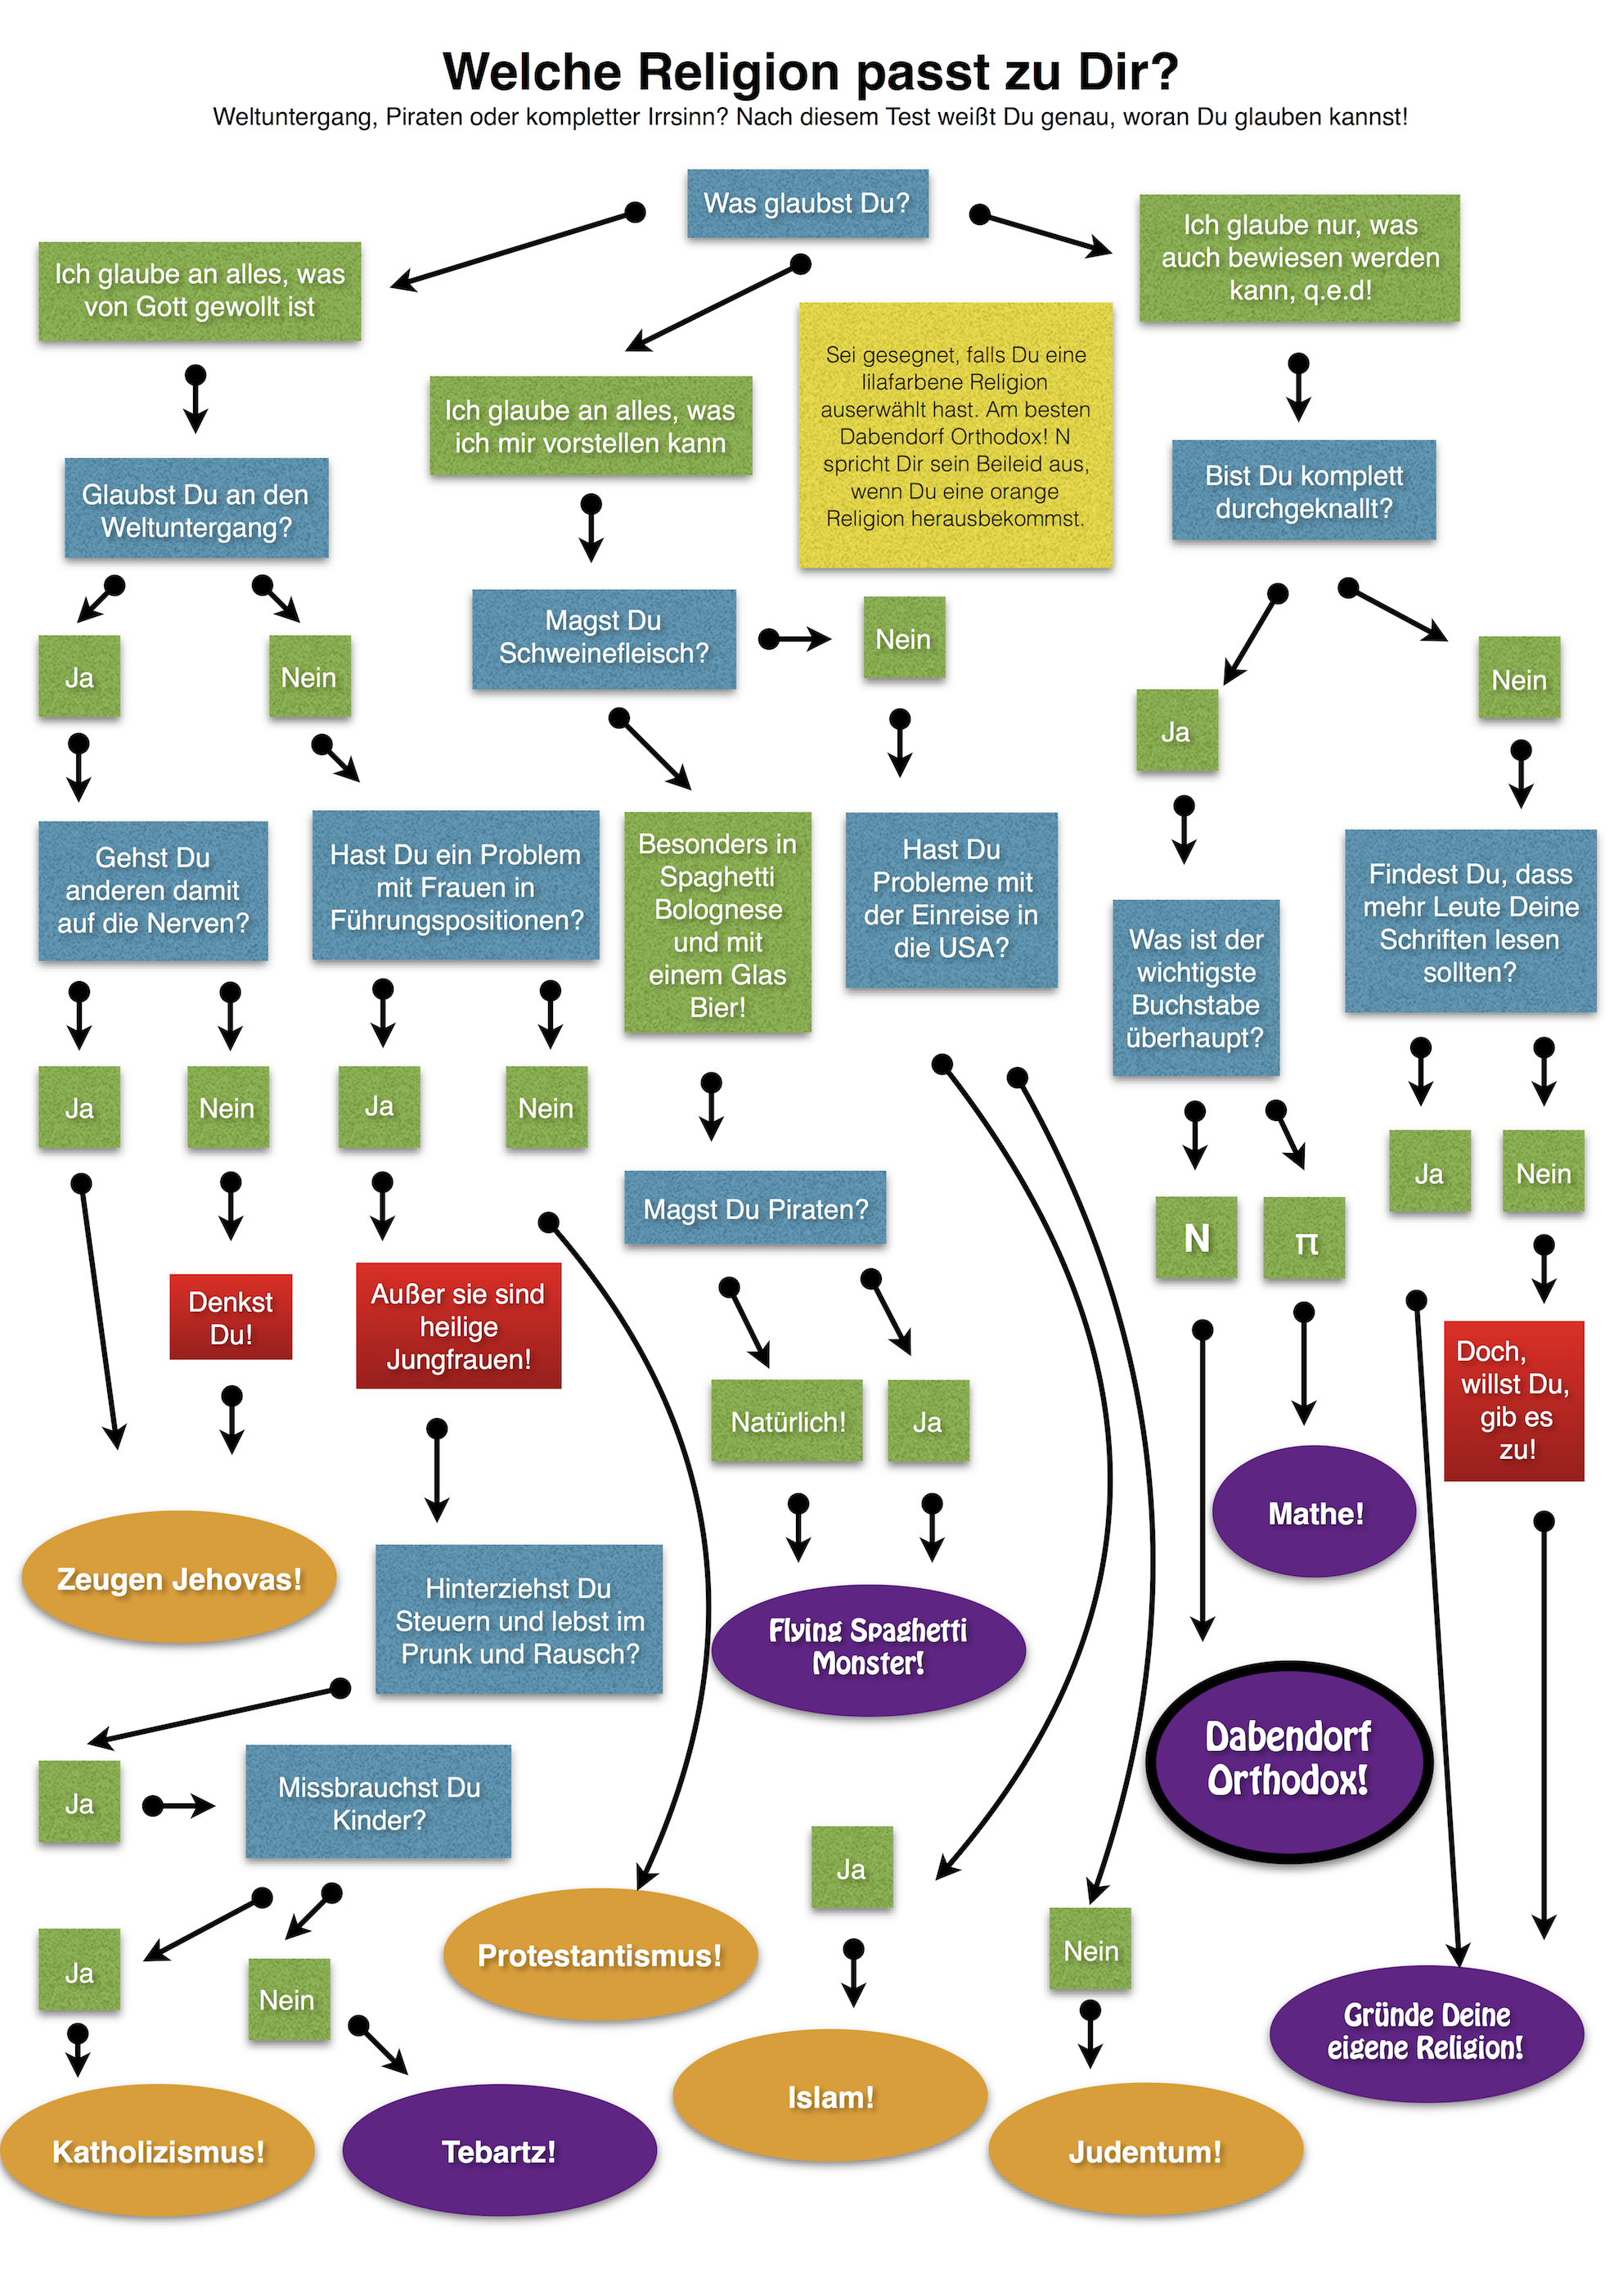
\includegraphics[width=1\textwidth]{bilder/Anhang_Religionsfrage}
\end{center}
\vspace*{\fill}

%Wie viel N
%Kreuzworträtsel?

%================
%\restoregeometry

%\newpage
%\glsaddall
%\printglossary[nonumberlist]

\end{document}